\documentclass[oneside]{book}

%%%%%%%%%%%%%%%%%%%%%%%%%%%%%%%%%%%%%%%%%%%%%
% PACKAGES
%%%%%%%%%%%%%%%%%%%%%%%%%%%%%%%%%%%%%%%%%%%%%

% STANDARD

\usepackage{etoolbox}
\usepackage{subcaption}
\usepackage{float}
\usepackage{xparse}
\usepackage{xstring}
\usepackage{enumitem}
\usepackage{graphicx}
\usepackage{diagbox}
\usepackage{listings}
\usepackage{rotating} %sideways environment
\usepackage[toc,page]{appendix}
\usepackage{pdflscape} % to use landscape pages
\usepackage{afterpage} % to put tables in landscape pages https://tex.stackexchange.com/a/19021/145331

% PROOF READING

\usepackage[T1]{fontenc}
\usepackage[utf8]{inputenc}
\usepackage[english]{babel}

% URL WITHIN THE PDF

\usepackage{hyperref}

% BIBLIOGRAPHY

\usepackage[nottoc,numbib]{tocbibind}

% TABLES

\usepackage{booktabs}
\usepackage{makecell}
\usepackage{longtable}



% SYMBOLS

\usepackage{pifont}
\usepackage{fontawesome}
\usepackage{textcomp} %TM

% URL

\usepackage{url}

% WARNING NOTES

\usepackage{mdframed}





% TIKZ

\usepackage{tikz}
\usetikzlibrary{arrows.meta, matrix, arrows,automata,positioning}

% FONTS AND COLORS

\usepackage{xcolor}
\usepackage{cancel}

% THEOREMS & MATHS

\usepackage{amsmath}
\usepackage{amsthm}
\usepackage{amssymb}
\usepackage{mathtools}

% ALGORITHMS

\usepackage[ruled,vlined,linesnumbered]{algorithm2e}

% GLOSSARIES

\usepackage[toc,acronym,style=index]{glossaries}
\usepackage[postdot]{glossaries-extra}

%%%%%%%%%%%%%%%%%%%%%%%%%%%%%%%%%%%%%%%%%%%%%
% IMPORTS OF CUSTOM COMMANDS
%%%%%%%%%%%%%%%%%%%%%%%%%%%%%%%%%%%%%%%%%%%%%

\usepackage{calculator}

%%%%%%%%%%%%%%%%%%%%%%%%%%%%%%%%%%%%%%%%%%%%%
% REFERENCES
%%%%%%%%%%%%%%%%%%%%%%%%%%%%%%%%%%%%%%%%%%%%%

\makeatletter

% Add a reference to a section
% param1 the label of the section
\NewDocumentCommand{\lstref}{m}{%
    Listing \ref{#1}%
}

% Add a reference to a section
% param1 the label of the section
\NewDocumentCommand{\listingref}{m}{%
    Listing \ref{#1}%
}


% Add a reference to a subsubsection
% param1 the label of the subsubsection
\NewDocumentCommand{\subsubsectionref}{m}{%
    Sub Sub Section \ref{#1}%
}

% Add a reference to a section
% param1 the label of the section
\NewDocumentCommand{\sectionref}{m}{%
    Section \ref{#1}%
}

% Add a reference to a equation
% param1 the label of the equation
\NewDocumentCommand{\equationref}{m}{%
    Equation \eqref{#1}%
}

% Add a reference to a algorithm line
% param1 the label of the algorithm line
\NewDocumentCommand{\alglineref}{m}{%
    Line \ref{#1}%
}

% Add a reference to a algorithm line
% param1 the label of the algorithm where piece starts
% param1 the label of the algorithm where priece ends
\NewDocumentCommand{\alglinesref}{m m}{%
    Lines \ref{#1}--\ref{#2}%
}

% Add a reference to an algorithm
% param1 the label of the algorithm
\NewDocumentCommand{\algref}{m}{%
    Algorithm \ref{#1}%
}

% Add a reference to a definition
% param1 the label of the definition
\NewDocumentCommand{\defref}{m}{%
    Definition \ref{#1}%
}

% Add a reference to a definition
% param1 the label of the first definition
% param2 the label of the second definition
\NewDocumentCommand{\defsref}{m m}{%
    Definitions \ref{#1}--\ref{#2}%
}

% Add a reference to a figure
% param1 the label of the figure
\NewDocumentCommand{\figref}{m}{%
    Figure \ref{#1}%
}

% Add a reference to a range of figure
% param1 the label of the first figure in the range (inclusive)
% param2 the label of the last figure in the range (inclusive)
\NewDocumentCommand{\figsref}{m m}{%
    Figures \ref{#1}--\ref{#2}%
}


\NewDocumentCommand{\r@figrefs}{m}{%
    \@ifnextchar\bgroup{, \ref{#1}\r@figrefs}{ and \ref{#1}}%
}
% Add a reference to a figure
% param1 the label of the figure
\NewDocumentCommand{\figrefs}{m}{%
    Figures \ref{#1}\r@figrefs%
}

% Add a reference to a table
% param1 the label of the table
\NewDocumentCommand{\tblref}{m}{%
    Table \ref{#1}%
}

% Add a reference to a theorem
% param1 the label of the table
\NewDocumentCommand{\thmref}{m}{%
    Theorem \ref{#1}%
}

% Add a reference to a lemma
% param1 the label of the lemma
\NewDocumentCommand{\lemmaref}{m}{%
    Lemma \ref{#1}%
}

% Add a reference to an example
% param1 the label of the example
\NewDocumentCommand{\exampleref}{m}{%
    Example \ref{#1}%
}

%%%%%%%%%%%%%%%%%%%%%%%%%%%%%%%%%%%%%%%%%%%%%
% EXAMPLE
%%%%%%%%%%%%%%%%%%%%%%%%%%%%%%%%%%%%%%%%%%%%%

\theoremstyle{definition}
\newtheorem{example}{Example}[section]

%%%%%%%%%%%%%%%%%%%%%%%%%%%%%%%%%%%%%%%%%%%%%
% USEFUL COMMANDS
%%%%%%%%%%%%%%%%%%%%%%%%%%%%%%%%%%%%%%%%%%%%%

%DOES NOT WORK
\NewDocumentEnvironment{verticalAlign}{+b}{%
    \topskip0pt%
    \vspace*{\fill}%
    {#1}%
    \vspace*{\fill}%
}{%
}

% Indent a body of text
% param1 dimension representing the space you want to indent
% param2 body actual content to put in the indented wall of text
\NewDocumentEnvironment{indentText}{O{3cm} +b}{%
    \begin{minipage}{\dimexpr\textwidth-#1}%
        #2%
        \xdef\tpd{\the\prevdepth}%
    \end{minipage}%
}{%
}

% Put a definition block in the text
%
% param1 the definition name. If not specified we won't have a definition
% param2 the label we want this definition to have. Input of \label. If not specified we won't put the \label command
% param3 the content of the definition
% \NewDocumentEnvironment{definition}{o o +b}{%
%     %BEGIN
%     \IfNoValueTF{#1}{%
%         \begin{theorem}%
%     }{%
%         \begin{theorem}[#1]%
%     }%
%     \IfNoValueF{#2}{%
%         \label{#2}%
%     }%
%     #2%
%     \end{theorem}%
% }{%
%     %END
% }
%     \IfNoValueTF{#1}{%
%         \begin{theorem}
%     }{%
%     }%
% }

\NewDocumentCommand{\setFontSize}{m o m}{%
    \IfNoValueF{#2}{%
        \fontsize{#1}{#2}\selectfont#3%
    }{%
        % see https://texblog.org/2012/08/29/changing-the-font-size-in-latex/
        \MULTIPLY{#1}{1.2}{\setFont@baseline}%
        \fontsize{#1}{\setFont@baseline}\selectfont#3%
    }%
}

% Adds a todo embedded in the text (colored blue)
% param1: an optional star: if a star is present, we will put the todo as a footnote
% param2: the text to put
\NewDocumentCommand{\todo}{s m}{%
    \IfBooleanTF{#1}{%
        \footnote{\color{blue} #2}%
    }{%
        {\color{blue} #2}%
    }%
}

%Adds a todo as a footnoe
\NewDocumentCommand{\code}{m}{%
    \texttt{#1}%
}

% draw a square.
% param1: fill color red!50
% param2: border color (default to black)
\NewDocumentCommand{\drawFilledSquare}{m O{black}}{%
    \begin{tikzpicture}%
        \node [rectangle,draw={#2},fill={#1}] (m) at (0,0) {};%
    \end{tikzpicture}%
}

% print a computer science ordered pair
% param1 first element of the pair
% param2 second element of the pair
\NewDocumentCommand{\paircs}{m m}{%
    \wrapMath{\langle {#1}, {#2} \rangle }%
}

\NewDocumentEnvironment{coloredBlock}{m O{blue} O{white}}{%
\setbeamercolor{block title}{bg=#2, fg=#3}
    \begin{block}{#1}%
}{%
    \end{block}%
}

\NewDocumentCommand{\stacksymbols}{m m}{%
    \wrapMath{\stackrel{\mathclap{#1}}{#2}}%
}

\NewDocumentCommand{\bigO}{m}{%
    \wrapMath{\mathcal{O}(#1)}%
}

\NewDocumentCommand{\nil}{}{%
    \texttt{NIL}%
}

\NewDocumentCommand{\doublePlus}{}{%
    \ifmmode{+\!\!+}\else{$+\!\!+$}\fi%
}

\NewDocumentCommand{\isInMath}{m m}{%
    \ifmmode{#1}\else{#2}\fi%
}

\NewDocumentCommand{\wrapMath}{m}{%
    \ifmmode{#1}\else{$#1$}\fi%
}

%apply double quotes on the parameter
% param1 the text to wrap quote
\NewDocumentCommand{\dquote}{m}{%
    ``{#1}''%
}

\NewDocumentCommand{\squote}{m}{%
    \isInMath%
        {\mbox{`}{#1}\mbox{'}}%
        {`{#1}'}%
}

%%%%%%%%%%%%%%%%%%%%%%%%%%%%%%%%%%%%%%%%%%%%%
% SYMBOLS
%%%%%%%%%%%%%%%%%%%%%%%%%%%%%%%%%%%%%%%%%%%%%

% draw a "v" representing a checkbox which has been checked
\NewDocumentCommand{\checked}{}{%
\tikz\fill[scale=0.4](0,.35) -- (.25,0) -- (1,.7) -- (.25,.15) -- cycle;%
}

% draw a "x" representing a checkbox which has been checked
\NewDocumentCommand{\unchecked}{}{%
\tikz\fill[scale=0.4]%
    (-0.35,+0.35) -- (+0.00,+0.07) --%
    (+0.40,+0.40) -- (+0.07,+0.00) --%
    (+0.35,-0.35) -- (+0.00,-0.07) --%
    (-0.40,-0.40) -- (-0.07,+0.00) --%
    cycle;%
}

%%%%%%%%%%%%%%%%%%%%%%%%%%%%%%%%%%%%%%%%%%%%%
% ACRONYM
%%%%%%%%%%%%%%%%%%%%%%%%%%%%%%%%%%%%%%%%%%%%%

\NewDocumentCommand{\eg}{}{%
    e.g.,%
}

\NewDocumentCommand{\ie}{}{%
    i.e.,%
}

\NewDocumentCommand{\st}{}{%
    s.t.%
}

\NewDocumentCommand{\wrt}{}{%
    w.r.t.%
}
\RenewDocumentCommand{\iff}{}{%
    \textit{iff}%
}

% see https://tex.stackexchange.com/a/369691/145331
\let\@oldcite\cite
\renewcommand*\cite[1]{~\@oldcite{#1}}


\makeatother

% Commands which are just alias for common latex operations

%%%%%%%%%%%%%%%%%%%%%%%%%%%%%%%%%%%%%%%%%%%%%
% PUT SOMETHING ON ITS OWN LANDSCAPE PAGE
%%%%%%%%%%%%%%%%%%%%%%%%%%%%%%%%%%%%%%%%%%%%%

\NewDocumentEnvironment{singlelandscape}{+b}{%
    \afterpage{%
        \clearpage% Flush earlier floats (otherwise order might not be correct)
        \thispagestyle{empty}% empty page style (?)
        \begin{landscape}% Landscape page
            {#1}%
        \end{landscape}%
        \clearpage% Flush page
    }%
}{%
}

%%%%%%%%%%%%%%%%%%%%%%%%%%%%%%%%%%%%%%%%%%%%%
% WARNING AND NOTES
%%%%%%%%%%%%%%%%%%%%%%%%%%%%%%%%%%%%%%%%%%%%%

% Show an attention box. The body of the environment is the body of the box 
\NewDocumentEnvironment{attention}{}{%
    \par%
        \begin{mdframed}[linewidth=3pt,linecolor=red]%
            \begin{list}{}{\leftmargin=1cm \labelwidth=\leftmargin}%
                \item[\Large\faBomb]%
}{%
            \end{list}%
        \end{mdframed}%
    \par
}

% Show a warning box. The body of the environment is the body of the box
\NewDocumentEnvironment{warning}{}{%
    \par%
        \begin{mdframed}[linewidth=3pt,linecolor=orange]%
            \begin{list}{}{\leftmargin=1cm \labelwidth=\leftmargin}%
                \item[\Large\faWarning]%
}{%
            \end{list}%
        \end{mdframed}%
    \par
}

% Show an note box. The body of the environment is the body of the box
\NewDocumentEnvironment{info}{}{%
    \par%
        \begin{mdframed}[linewidth=3pt,linecolor=blue]%
            \begin{list}{}{\leftmargin=1cm \labelwidth=\leftmargin}%
                \item[\Large\faBook]%
}{%
            \end{list}%
        \end{mdframed}%
    \par
}

% Alias of "info"
\NewDocumentEnvironment{note}{}{%
    \par%
        \begin{mdframed}[linewidth=3pt,linecolor=blue]%
            \begin{list}{}{\leftmargin=1cm \labelwidth=\leftmargin}%
                \item[\Large\faBook]%
}{%
            \end{list}%
        \end{mdframed}%
    \par
}

%%%%%%%%%%%%%%%%%%%%%%%%%%%%%%%%%%%%%%%%%
% FLOATS
%%%%%%%%%%%%%%%%%%%%%%%%%%%%%%%%%%%%%%%%%

%Setup the a horizontal page instead of the classic portait page
\NewDocumentCommand{\insertFigure}{}{}
\NewDocumentEnvironment{horizontalpage}{+b}{%
    \begin{sidewaysfigure}%
        #1%
    \end{sidewaysfigure}%
}{%
}

%%%%%%%%%%%%%%%%%%%%%%%%%%%%%%%%%%%%%%%%%
% TEX COMMONS
%%%%%%%%%%%%%%%%%%%%%%%%%%%%%%%%%%%%%%%%%

% Write something in italic. Alias of \textit
% param1 the text to write in italic
\NewDocumentCommand{\italic}{m}{%
    \textit{#1}%
}

%%%%%%%%%%%%%%%%%%%%%%%%%%%%%%%%%%%%%%%%%
% GLOSSARIES
%%%%%%%%%%%%%%%%%%%%%%%%%%%%%%%%%%%%%%%%%

% Display the given acronym 
% param1 name of the acronym to print
\NewDocumentCommand{\acronymRef}{m}{%
   \gls{#1}%
}


% Display the given acronym 
% param1 name of the acronym to print
\NewDocumentCommand{\acrref}{m}{%
   \gls{#1}%
}

% Display a glossary entry with the first letter as miniscule.
%This is just a more rememberable alias of \gls
% param1 name of the glossary entry to cite. 
\NewDocumentCommand{\glossaryRef}{m}{%
    \gls{#1}%
}

% Display a glossary entry with the first letter as capital.
%This is just a more rememberable alias of \Gls
% param1 name of the glossary entry to cite. 
\NewDocumentCommand{\GlossaryRef}{m}{%
    \Gls{#1}%
}

% Display a glossary entry with the first letter as miniscule.
%This is just a more rememberable alias of \gls
% param1 name of the glossary entry to cite. 
\NewDocumentCommand{\glsref}{m}{%
    \gls{#1}%
}

% Display a glossary entry with the first letter as capital.
%This is just a more rememberable alias of \Gls
% param1 name of the glossary entry to cite. 
\NewDocumentCommand{\Glsref}{m}{%
    \Gls{#1}%
}



%%%%%%%%%%%%%%%%%%%%%%%%%%%%%%%%%%%%%%%%
% NAMES
%%%%%%%%%%%%%%%%%%%%%%%%%%%%%%%%%%%%%%%%

\NewDocumentCommand{\true}{}{%
    \code{true}%
}

\NewDocumentCommand{\false}{}{%
    \code{false}%
}

\NewDocumentCommand{\NPComplete}{}{%
    \code{NP}-Complete%
}

\NewDocumentCommand{\NPHard}{}{%
    \code{NP}-Hard%
}

\NewDocumentCommand{\NPHardness}{}{%
    \code{NP}-Hardness%
}

%define default listing settings

\lstset{%
    postbreak=\mbox{\textcolor{red}{$\hookrightarrow$}\space},%
    frame={single},%
    breaklines={true},%
    captionpos={b}%
}

%%%%%%%%%%%%%%%%%%%%%%%%%%%%%%%%%%%%%%%%%%
% XML
%%%%%%%%%%%%%%%%%%%%%%%%%%%%%%%%%%%%%%%%%%

\definecolor{xmlgray}{rgb}{0.4,0.4,0.4}
\definecolor{xmldarkblue}{rgb}{0.0,0.0,0.6}
\definecolor{xmlcyan}{rgb}{0.0,0.6,0.6}


\lstdefinelanguage{xml}{
  basicstyle=\footnotesize\ttfamily,
  columns=fullflexible,
  showstringspaces=false,
  commentstyle=\color{xmlgray}\upshape,
    %
  morestring=[b]",
  morestring=[s]{>}{<},
  morecomment=[s]{<?}{?>},
  stringstyle=\color{black},
  identifierstyle=\color{xmldarkblue},
  keywordstyle=\color{xmlcyan},
  morekeywords={xmlns,version,type}% list your attributes here
}

%%%%%%%%%%%%%%%%%%%%%%%%%%%%%%%%%%%%%%%%%%
% JSON
%%%%%%%%%%%%%%%%%%%%%%%%%%%%%%%%%%%%%%%%%%

%define listing for json language
% see https://tex.stackexchange.com/a/433961/145331
\definecolor{eclipseStrings}{RGB}{42,0.0,255}
\definecolor{eclipseKeywords}{RGB}{127,0,85}
\colorlet{numb}{magenta!60!black}

\lstdefinelanguage{json}{
    basicstyle=\footnotesize\ttfamily,
    commentstyle=\color{eclipseStrings}, % style of comment
    stringstyle=\color{eclipseKeywords}, % style of strings
    numbers=left,
    numberstyle=\scriptsize,
    stepnumber=1,
    numbersep=8pt,
    showstringspaces=false,
    breaklines=true,
    frame={single},
    %backgroundcolor=\color{gray}, %only if you like
    string=[s]{"}{"},
    comment=[l]{:\ "},
    morecomment=[l]{:"},
    literate=
        *{0}{{{\color{numb}0}}}{1}
         {1}{{{\color{numb}1}}}{1}
         {2}{{{\color{numb}2}}}{1}
         {3}{{{\color{numb}3}}}{1}
         {4}{{{\color{numb}4}}}{1}
         {5}{{{\color{numb}5}}}{1}
         {6}{{{\color{numb}6}}}{1}
         {7}{{{\color{numb}7}}}{1}
         {8}{{{\color{numb}8}}}{1}
         {9}{{{\color{numb}9}}}{1}
}

%define default listing settings

%%%%%%%%%%%%%%%%%%%%%%%%%%%%%%%%%%%%%%%%%%
% EBNF
%%%%%%%%%%%%%%%%%%%%%%%%%%%%%%%%%%%%%%%%%%

%define listing for RMS language
% see https://tex.stackexchange.com/a/433961/145331
\definecolor{eclipseStrings}{RGB}{42,0.0,255}
\definecolor{eclipseKeywords}{RGB}{127,0,85}
\colorlet{numb}{magenta!60!black}

\lstdefinelanguage{ebnf}{%
    postbreak=\mbox{\textcolor{red}{$\hookrightarrow$}\space},%
    frame={single},%
    breaklines={true},%
    captionpos={b},%
    basicstyle=\footnotesize\ttfamily,%
    commentstyle=\color{eclipseStrings}, % style of comment
    stringstyle=\color{eclipseKeywords}, % style of strings
    numbers=left,%
    numberstyle=\scriptsize,%
    stepnumber=1,%
    numbersep=8pt,%
    showstringspaces=false,%
    %backgroundcolor=\color{gray}, %only if you like
    morestring=[s]{"}{"},%
    morestring=[s]{'}{'},%
    comment=[l]{:\ "},%
    morecomment=[l]{:"},%
    morekeywords={<-}%
}

%%%%%%%%%%%%%%%%%%%%%%%%%%%%%%%%%%%%%%%%%%
% RMS
%%%%%%%%%%%%%%%%%%%%%%%%%%%%%%%%%%%%%%%%%%

\lstdefinelanguage{rms}{%
    postbreak=\mbox{\textcolor{red}{$\hookrightarrow$}\space},%
    frame={single},%
    breaklines={true},%
    captionpos={b},%
    basicstyle=\footnotesize\ttfamily,%
    commentstyle=\color{eclipseStrings}, % style of comment
    stringstyle=\color{eclipseKeywords}, % style of strings
    numbers=left,%
    numberstyle=\scriptsize,%
    stepnumber=1,%
    numbersep=8pt,%
    showstringspaces=false,%
    %backgroundcolor=\color{gray}, %only if you like
    string=[s]{"}{"},%
    comment=[l]{:\ "},%
    morecomment=[l]{:"},%
    morekeywords={\#define,\#include\_drs,\#const,if,else,endif,elseif}%
}
\NewDocumentCommand{\aoe}{}{%
    Age of Empires II: DE%
}

\NewDocumentCommand{\steam}{}{%
    Steam%
}

\NewDocumentCommand{\genie}{}{%
    Advance Genie Editor%
}

\NewDocumentCommand{\aoeexedir}{}{%
    \code{\aoe{} Exe}%
}

\NewDocumentCommand{\aoehomedir}{}{%
    \code{\aoe{} Home}%
}

\NewDocumentCommand{\aoeweirdnumberdir}{}{%
    \code{\aoe{} SteamId}%
}

\NewDocumentCommand{\aoehomelocaldir}{}{%
    \code{\aoe{} Local Mod}%
}

\NewDocumentCommand{\term}{m}{%
    {#1}%
}

%%%%%%%%%%%%%%%%%%%%%%%%%%%%%%%%%%%%%%%%%%%%%
% GEOMTRIES
%%%%%%%%%%%%%%%%%%%%%%%%%%%%%%%%%%%%%%%%%%%%%

\renewcommand{\dblfloatpagefraction}{0.95}
\renewcommand{\dbltopfraction}{1}
\renewcommand{\topfraction}{1}
\renewcommand{\textfraction}{0.0}
\renewcommand{\floatpagefraction}{1}

%%%%%%%%%%%%%%%%%%%%%%%%%%%%%%%%%%%%%%%%%%%%%
% DOCUMENT FRONT PAGE
%%%%%%%%%%%%%%%%%%%%%%%%%%%%%%%%%%%%%%%%%%%%%
\title{Age of Empires DE, a tutorial for modding}
\author{Koldar}
\date{\today}





%%%%%%%%%%%%%%%%%%%%%%%%%%%%%%%%%%%%%%%%%%%%%
% THEOREMS
%%%%%%%%%%%%%%%%%%%%%%%%%%%%%%%%%%%%%%%%%%%%%

%declare theorem, definitions, corollary, lemmas
\newtheorem{theorem}{Theorem}[section]
\newtheorem{corollary}{Corollary}[theorem]
\newtheorem{lemma}[theorem]{Lemma}

\newtheorem{definition}{Definition}[section]

%%%%%%%%%%%%%%%%%%%%%%%%%%%%%%%%%%%%%%%%%%%%%
% GLOSSARIES
%%%%%%%%%%%%%%%%%%%%%%%%%%%%%%%%%%%%%%%%%%%%%

% see http://tug.ctan.org/macros/latex/contrib/glossaries/glossariesbegin.pdf
\setabbreviationstyle[acronym]{long-short}% glossaries-extra.sty only

\newglossary*{terms}{Terms}
%acronym glossary is automatically added by flag acronym \newglossary[alg]{acronym}{acr}{acn}{\acronymname}

\makeglossaries
\newglossaryentry{personalcomputer}
{
    type={terms},
    name={Personal Computer},
    description={A general purpose machine}
}

%\newglossaryentry{}
%{
%	type={terms},
%	name={},
%	description={}
%}

\newglossaryentry{intellisense}
{
    type={terms},
    name={intellisense},
    description={In Visual Studio and similar product, IntelliSense is a code-completion aid developed by Microsoft that includes a number of features: List Members, Parameter Info, Quick Info, and Complete Word. These features help you to learn more about the code you're using, keep track of the parameters you're typing, and add calls to properties and methods with only a few keystrokes.\cite{intellisense:2020}}
}

\newglossaryentry{activeX}
{
    type={terms},
    name={ActiveX},
    description={Much like Java Applets, ActiveX controls are small apps that allow websites to provide content such as videos and games. They also let you interact with content like toolbars and stock tickers when you browse the web.\cite{activeX}}
}

\newglossaryentry{nuget}
{
    type={terms},
    name={NuGet},
    description={Maven-like repository where you can automatically install C\# dependencies.}
}



% \newacronym{PC}{PC}{Personal Computer}


\newacronym{DDS}{DDS}{DirectDraw Surface}

\newacronym{PNG}{PNG}{Portable Network Graphics}

\newacronym{UI}{UI}{User Interface}

\newacronym{URL}{URL}{Uniform Resource Locator}

\newacronym{DAT}{DAT}{DATa}

\newacronym{PC}{PC}{Personal Computer}
\newacronym{JSON}{JSON}{JavaScript Object Notation}
\newacronym{HTTP}{HTTP}{Hyper-Text transfer Protocol}
\newacronym{DLL}{DLL}{Dynamic Link Library}
\newacronym{TCP}{TCP}{Transmission Control Protocol}
\newacronym{IP}{IP}{Internet Protocol}
\newacronym{NAT}{NAT}{Network Address Translator}
\newacronym{REST}{REST}{REpresentational State Transfer}
\newacronym{RCP}{RCP}{Remote Call Procedure}
\newacronym{CSRF}{CSRF}{Cross Site Request Forgery}
\newacronym{GUID}{GUID}{Globally Unique IDentifier}
\newacronym{EXE}{EXE}{EXEcutable}
\newacronym{MSI}{MSI}{Microsoft Installer}

%%%%%%%%%%%%%%%%%%%%%%%%%%%%%%%%%%%%%%%%%%%%%
% MAIN DOCUMENT
%%%%%%%%%%%%%%%%%%%%%%%%%%%%%%%%%%%%%%%%%%%%%

\begin{document}

%see https://tex.stackexchange.com/a/13920/145331
\begin{titlepage}
    \centering
    \vfill
    {\bfseries\Large
        \makeatletter\@title\makeatother
        
        \vskip2cm

        \makeatletter\@author\makeatother
        
        \vskip2cm

        Version 1.0.0
        \\
    }    
    \vfill
    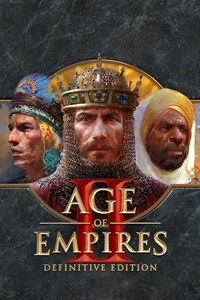
\includegraphics[width=0.5\textwidth]{src/images/logo}
    \vfill
    \vfill
    Date: \makeatletter\@date\makeatother
\end{titlepage}
\clearpage

\frontmatter

\tableofcontents
\clearpage

\listoffigures
\clearpage

%\listofalgorithms
%\clearpage
 
\listoftables
\clearpage

%\printunsrtglossaries
\printglossary[type=\acronymtype]
\clearpage

\chapter{About this report}

When writing this guide, the following convention are adopted.

Generally speaking, definitions of concepts are shown as:

\begin{definition}{Square root of a number}
    The square root of a number $x$ ($\sqrt{x}$) is defined as the number that, multiplied with itself, yield $x$.
\end{definition}

A note is something that adds context to a topic and is shown as below:

\begin{info}
    Default methods in C\# interfaces have been heavily inspired by java's default method implementation
\end{info}

A warning is something that you should be aware of.

\begin{warning}
    You shouldn't read a variable value before setting it.
\end{warning}

An attention contains information that, if not followed, will cause unexpected results;

\begin{attention}
    In C, don't read a variable value before setting it.
\end{attention}

Reference to the glossary are printed as below:

\glsref{personalcomputer} are used throughout the world.

Whole reference to the acronym table are shown as:

\acrref{PC} are used throughout the world.

Citation are shown as follows: in A* algorithm, we use $f=g+h$ to estimate search states\cite{hart1968-astar}.


\mainmatter
\chapter{Introduction}

This guide helps you creating a new mod in \aoe{}: by reading this file, you should be able to create simple mods. I have written this guide when I started my \aoe{} modding experience and contains all the information I have gathered while scouting the internet. I tried to include the most important information, but I have decided to leave some other (albeit relevant) information out from this document. Hence, the data presented here may be lacking or missing.

Note that this guide focuses its attention on \aoe{}, while other version of the game (\eg{} Age of Conqueror or HD version) are explicitly not considered whatsoever: this usually means that some functions or characteristics may not be available in such game versions. The work here has been done in order to fix the stable bug from \dquote{Persistent Corpses} data mod\cite{steamid:2019} and in order to create more team maps where me and my friend can play in.

All code (alongside the source code of this document) is available at \url{https://github.com/Koldar/aoe-mod-tutorial}: please open an issue whenever you find any typos, missing references of false information.


\chapter{Background and Related Works}


\section{Maps}

\begin{definition}
    A map is said to be \textbf{nomad} when the players will start with no towncenter, and some villagers. Each player is required to create a town center wherever she desires.
\end{definition}

\begin{definition}
    A map is said to be \textbf{michi} the players will be separated by forest.
\end{definition}

Cliffs (see \defref{def:cliff}) are another element on the map. A cliff is shown in \figref{fig:cliff}

\begin{definition}\label{def:cliff}
    A cliff is an untraversable element of the map. Units on the cliff gain a strategic advantage \wrt{} unit under the cliff.
\end{definition}

\begin{figure}[ht]
    \centering
    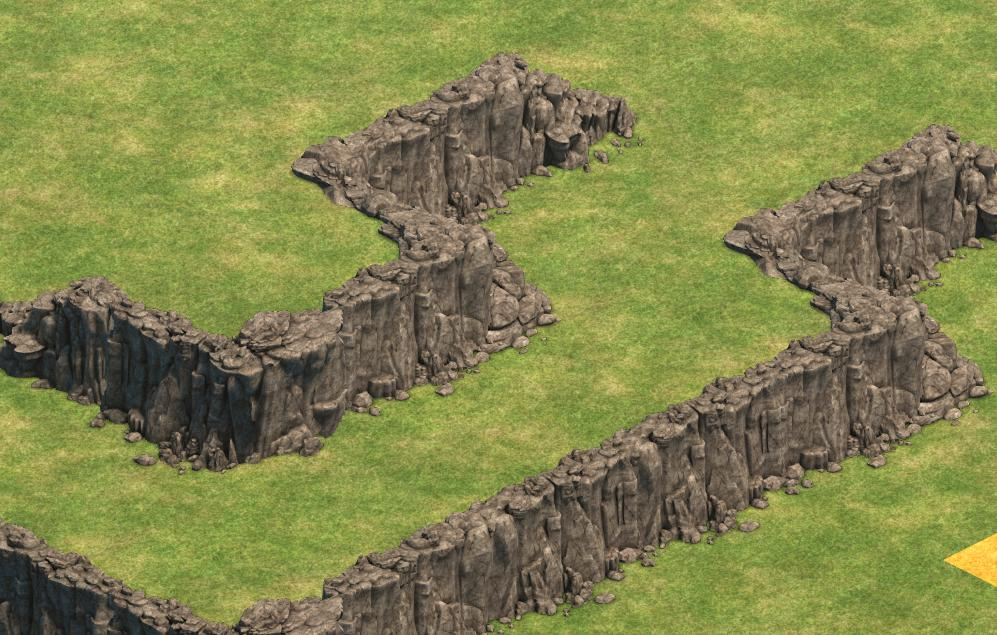
\includegraphics[width=0.8\textwidth]{src/images/cliffs}
    \caption{Example of a cliff in a map.}
    \label{fig:cliff}
\end{figure}

Maps have fixed \textbf{sizes}, which are shown in \tblref{tbl:size}\cite{zetnus:2015}.

\begin{table}[ht]
    \centering
    \begin{tabular}{llll}
        \toprule
        Size & Tiles on Sides & Total tiles & Area ratio to 100x100 map \\
        \midrule
        Tiny        & 120x120              & 14400           & 1.4 \\
        Small       & 144x144              & 20736           & 2.1 \\
        Medium      & 168x168              & 28224           & 2.8 \\
        Large       & 200x200              & 40000           & 4.0 \\
        Huge        & 220x220              & 48400           & 4.8 \\
        Gigantic    & 240x240              & 57600           & 5.8 \\
        Ludicruous  & 480x480              & 230400          & 23.0 \\
        \bottomrule
    \end{tabular}
    \caption{Allowed map sizes.}
    \label{tbl:size}
\end{table}

\subsection{Types of maps}

You can play \aoe{} on several different maps. A map can be played with a specific playstyle. The types of maps are the following ones:

\begin{itemize}
    \item Random Maps
    \item Death Match;
    \item Battle Royale;
    \item King of the Hill;
\end{itemize}

\figref{fig:aoe:maps} shows some maps available to play in \aoe{}.

\begin{figure}
    \begin{subfigure}{0.22\textwidth}
        \centering
        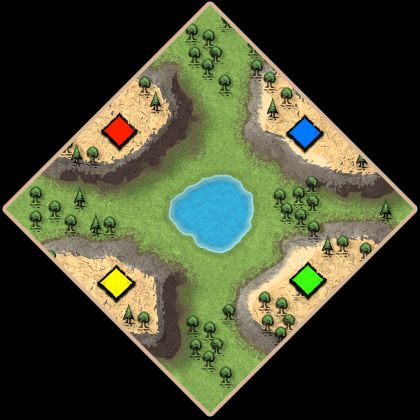
\includegraphics[width=1.0\textwidth]{src/images/maps/rm-acropolis}
        \caption{Acropolis}
    \end{subfigure}\quad%
    \begin{subfigure}{0.22\textwidth}
        \centering
        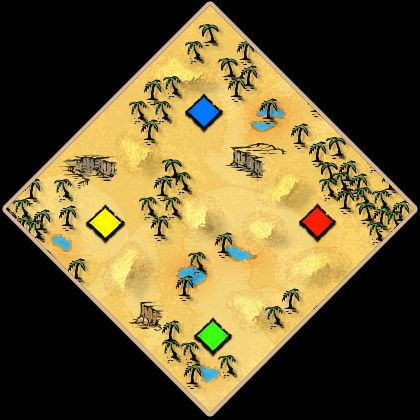
\includegraphics[width=1.0\textwidth]{src/images/maps/rm-arabia}
        \caption{Arabia}
    \end{subfigure}\quad%
    \begin{subfigure}{0.22\textwidth}
        \centering
        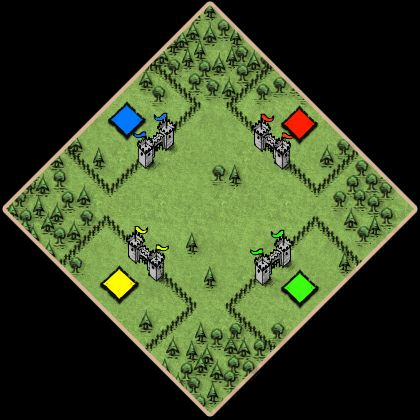
\includegraphics[width=1.0\textwidth]{src/images/maps/rm-arena}
        \caption{Arena}
    \end{subfigure}\quad%
    \begin{subfigure}{0.22\textwidth}
        \centering
        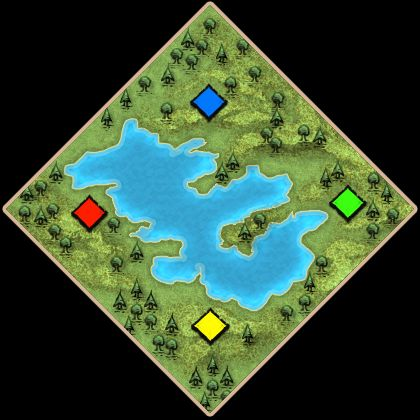
\includegraphics[width=1.0\textwidth]{src/images/maps/rm-baltic}
        \caption{Baltic}
    \end{subfigure}\\%
    %
    \begin{subfigure}{0.22\textwidth}
        \centering
        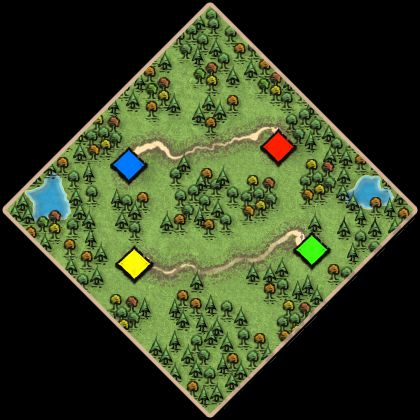
\includegraphics[width=1.0\textwidth]{src/images/maps/rm-black-forest}
        \caption{Black Forest}
    \end{subfigure}\quad%
    \begin{subfigure}{0.22\textwidth}
        \centering
        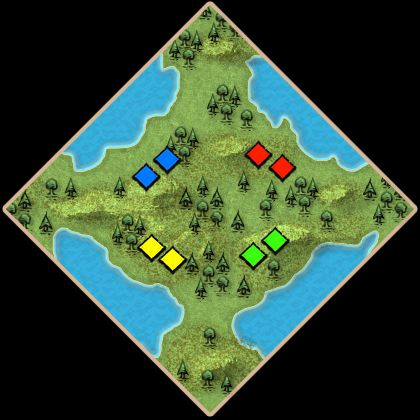
\includegraphics[width=1.0\textwidth]{src/images/maps/rm-budapest}
        \caption{Budapest}
    \end{subfigure}\quad%
    \begin{subfigure}{0.22\textwidth}
        \centering
        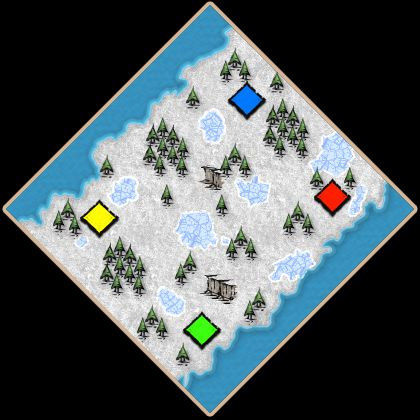
\includegraphics[width=1.0\textwidth]{src/images/maps/rm-scandinavia}
        \caption{Scandinavia}
    \end{subfigure}\quad%
    \begin{subfigure}{0.22\textwidth}
        \centering
        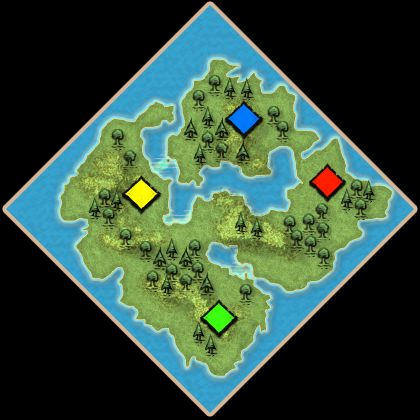
\includegraphics[width=1.0\textwidth]{src/images/maps/rm-continental}
        \caption{Continental}
    \end{subfigure}\\%
    % %
    % \begin{subfigure}{0.24\textwidth}
    %     \centering
    %     \includegraphics[1.0\textwidth]{src/images/maps/}
    %     \caption{}
    % \end{subfigure}%
    % \begin{subfigure}{0.24\textwidth}
    %     \centering
    %     \includegraphics[1.0\textwidth]{src/images/maps/}
    %     \caption{}
    % \end{subfigure}%
    % \begin{subfigure}{0.24\textwidth}
    %     \centering
    %     \includegraphics[1.0\textwidth]{src/images/maps/}
    %     \caption{}
    % \end{subfigure}%
    % \begin{subfigure}{0.24\textwidth}
    %     \centering
    %     \includegraphics[1.0\textwidth]{src/images/maps/}
    %     \caption{}
    % \end{subfigure}\\%
    % %
    % \begin{subfigure}{0.24\textwidth}
    %     \centering
    %     \includegraphics[1.0\textwidth]{src/images/maps/}
    %     \caption{}
    % \end{subfigure}%
    % \begin{subfigure}{0.24\textwidth}
    %     \centering
    %     \includegraphics[1.0\textwidth]{src/images/maps/}
    %     \caption{}
    % \end{subfigure}%
    % \begin{subfigure}{0.24\textwidth}
    %     \centering
    %     \includegraphics[1.0\textwidth]{src/images/maps/}
    %     \caption{}
    % \end{subfigure}%
    % \begin{subfigure}{0.24\textwidth}
    %     \centering
    %     \includegraphics[1.0\textwidth]{src/images/maps/}
    %     \caption{}
    % \end{subfigure}\\%
    % %
    % \begin{subfigure}{0.24\textwidth}
    %     \centering
    %     \includegraphics[1.0\textwidth]{src/images/maps/}
    %     \caption{}
    % \end{subfigure}%
    % \begin{subfigure}{0.24\textwidth}
    %     \centering
    %     \includegraphics[1.0\textwidth]{src/images/maps/}
    %     \caption{}
    % \end{subfigure}%
    % \begin{subfigure}{0.24\textwidth}
    %     \centering
    %     \includegraphics[1.0\textwidth]{src/images/maps/}
    %     \caption{}
    % \end{subfigure}%
    % \begin{subfigure}{0.24\textwidth}
    %     \centering
    %     \includegraphics[1.0\textwidth]{src/images/maps/}
    %     \caption{}
    % \end{subfigure}\\
    \caption{Examples of maps available in \aoe{}. Red, Yellow, Green and Blue diamond represents players positions. If a team game is played, Red and blue are allied against team yellow and green. A shoe represents a nomadic map. }
    \label{fig:aoe:maps}
\end{figure}
\chapter{Basics and Definitions}

The first thing is to install \aoe{}, for instance, via \steam{}\cite{Ozhara:2017}. After that, you need to identify \genie{} program: it is usually installed at \dquote{C:\textbackslash{}Program Files (x86)\textbackslash{}Steam\textbackslash{}steamapps\textbackslash{}common\textbackslash{}AoE2DE\textbackslash{}Tools\_Builds\textbackslash{}AdvancedGenieEditor3.exe}. Data mods are discourages\cite{yorok:2019}, hence you should create modes by replacing individual files and avoiding data modding whenever possible. We will refer to the folder \verb|C:\Program Files (x86)\Steam\steamapps\common\AoE2DE\| as \aoeexedir{}.

The mods you install from \aoe{} are available in a directory that usually is \verb|%HOMEPATH%\Games\Age of Empires 2 DE| (from here on dubbed \aoehomedir{}).
Within \aoehomedir{}, there should be a folder whose name is the user \textbf{steam id} (which is a big number) (from here on such a folder is dubbed as \aoeweirdnumberdir{})\cite{steamid:2019}. Within it, there is a folder called \verb|mods\subscribed| containing all the mods the user has subscribed to. Along side \dquote{subscribed} folder, there is a folder named \dquote{local} where local mods in development may be put (such a folder will be referred to as \aoehomelocaldir{}). The structure of \aoehomedir{} is shown in \lstref{verb1}.

\lstinputlisting[label=verb1,caption={Age of Empires home folder directory structure}, float, frame=ht]{src/codes/folder-structure.txt}

For example, \tblref{tbl:paths} shows all the involved paths for the modding.

\begin{table}[ht]
    \centering
    \small
    \begin{tabular}{ll}
        \toprule
        Path & Example \\
        \midrule
        \aoeexedir{}            & \code{C:\textbackslash{}Program Files (x86)\textbackslash{}Steam\textbackslash{}steamapps\textbackslash{}common\textbackslash{}AoE2DE\textbackslash{}} \\
        \aoehomedir{}           & \code{C:\textbackslash{}Users\textbackslash{}FooBar\textbackslash{}Games\textbackslash{}Age of Empires 2 DE} \\
        \aoeweirdnumberdir{}    & \code{C:\textbackslash{}Users\textbackslash{}FooBar\textbackslash{}Games\textbackslash{}Age of Empires 2 DE\textbackslash{}9823578647902347890} \\
        \bottomrule
    \end{tabular}
    \caption{Examples of important paths used in \aoe{}}
    \label{tbl:paths}
\end{table}

In the \dquote{mods} folder, there is a file called \code{mods-status.json} (an example of the content is shown in \lstref{verb2}).

\lstinputlisting[language=json,caption=Example of mods-status file,label=verb2, frame=ht]{src/codes/mods-status.json}

The json stored is a sequence of objects, each representing:

\begin{itemize}
    \item Checksum: MD5 of the mod?
    \item \textbf{Enable}: if \true{}, the mod is enabled, \false{} otherwise;
    \item Last Update: timestamp representing the number of milliseconds when the mod has been lastly updated;
    \item \textbf{Path}: path, relative to \aoeweirdnumberdir{} directory, where the specific mod is installed;
    \item \textbf{Priority}: priority used to load the mod;
    \item Publish Id: always 0?
    \item \textbf{Title}: name of the mod to show to the user;
    \item WorkShop Id: An id that uniquely identifies this mod on \url{www.ageofempires.com} site;
\end{itemize}


At high level \aoe{} install each mod by following \algref{alg:bootstrap}. 
After sorting out the enabled mods, the software \dquote{patches} the set of files specified by the mod path.
From the algorithm, it can be seen that the priority of each mod determine the order each mod is used. Priority may change the behavior is a mod $x$ relies on the installation of the mod $y$ (if $y.priority < x.priority$)\cite{Ozhara:2017}.

\begin{algorithm}
    \SetAlgoLined
    $mods \leftarrow$ Gather mods in \aoeweirdnumberdir{}\;
    $sortedmods \leftarrow$ Sort $mods$ by prioritzing mods with small priority\;
    \ForEach(mods subscribed){$m \in reversed(sortedmods)$}{
        \If{$\neg m.Enable$}{
            \textbf{continue}\;
        }
        Copy the files in \aoeweirdnumberdir{}\textbackslash{}mods\textbackslash{}$m.Path$ into \aoeexedir{}\;
    }
    Start \aoe{}\;
    \caption{\aoe{} mod boot strap algorithm}
    \label{alg:bootstrap}
\end{algorithm}
\chapter{Creating a basic mod (MWE)}

When developing a mod you should work in the directory \aoehomelocaldir{}.
Start by creating a folder with the same name as the mod you want to create. For this tutorial, we will create a mod that changes the background of the main menu: we will name such a folder \dquote{carcassone-menu}.

For this very reason we need to put the background image (in this case the one shown in \figref{fig:carcassonne})

\begin{figure}[ht]
    \centering
    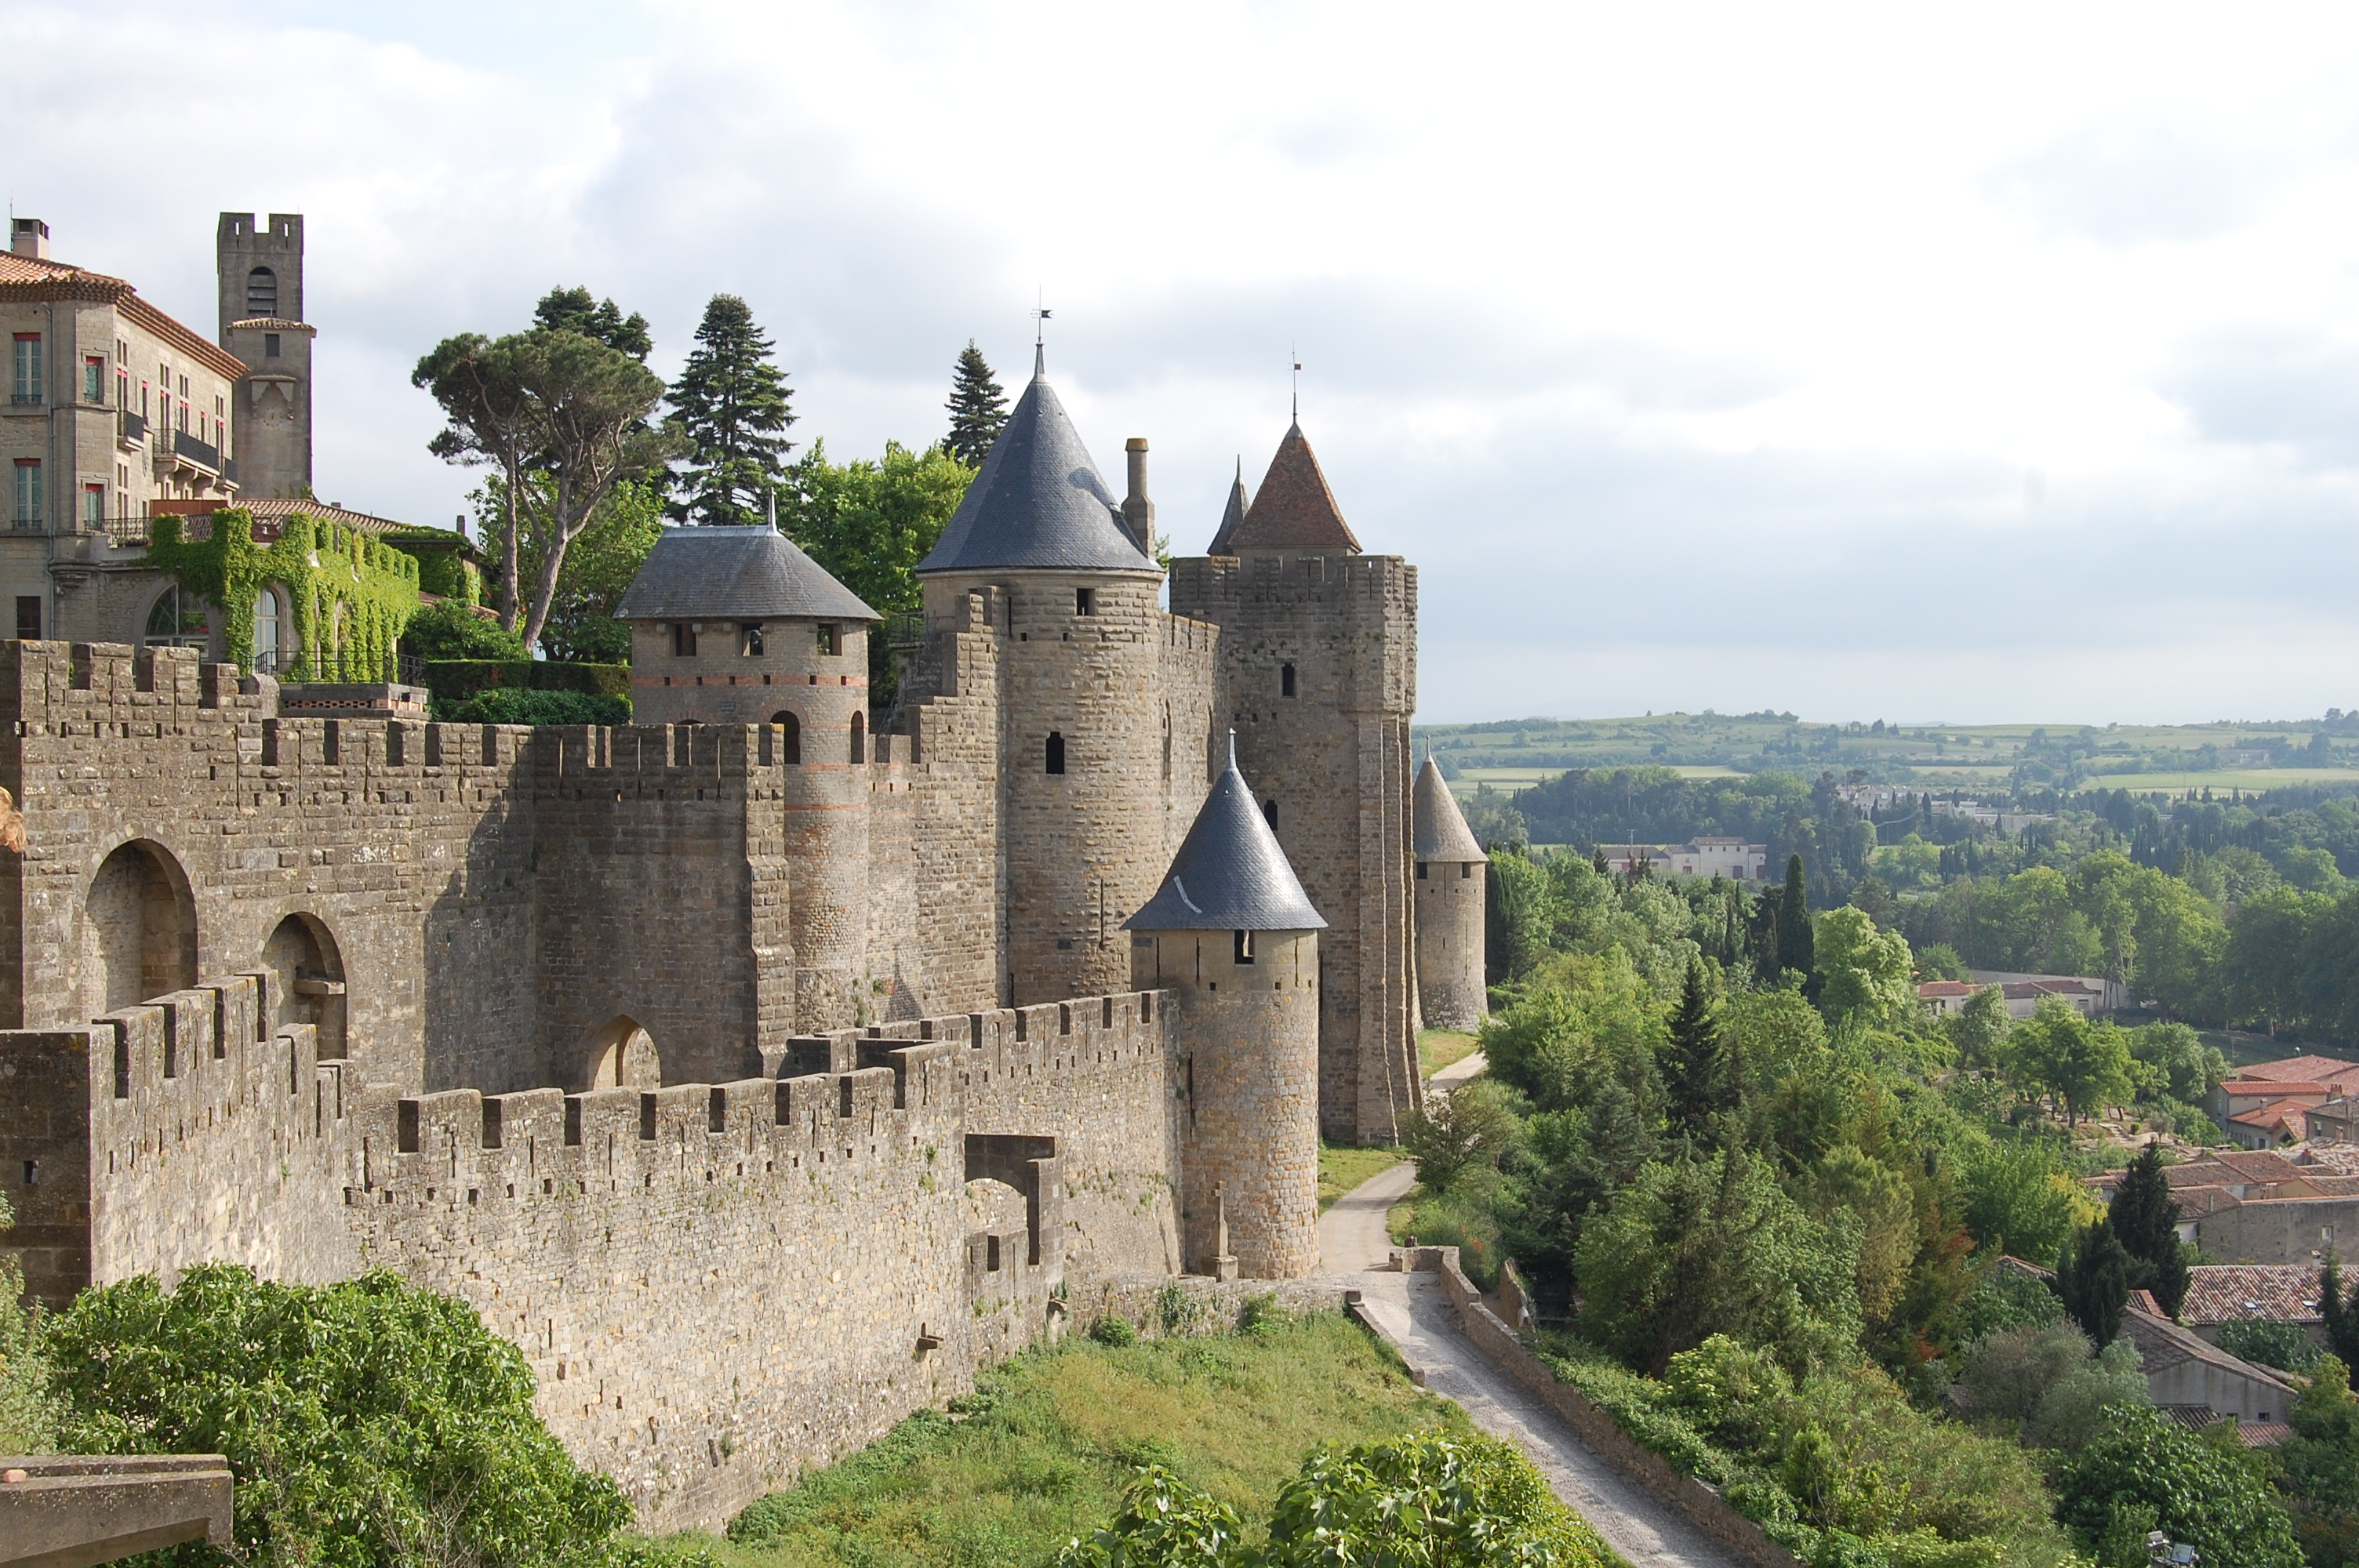
\includegraphics[width=1.0\textwidth]{src/images/carcassonne}
    \caption{Image to put as background}
    \label{fig:carcassonne}
\end{figure}

As shown in the Appendix \ref{chp:semantics}, the background image is specified (relative to \aoeexedir{}) in \code{widgetui/textures/backgrounds/mainmenu\_bg.dds}.
Hence, in the \dquote{carcassone-menu} folder, you need to create the subfolder \code{widgetui/textures/backgrounds/mainmenu\_bg}; then you need to put the Carcassone image, name it \dquote{mainmenu\_bg} (ensure that the image follows the \acrref{DDS} extension).

\lstinputlisting[label=verb3,caption={Carcassonne mod layout}, float, frame=ht]{src/codes/carcassonne-mod-layout.txt}

Aside the folders you have just created, you need two additional files that represents mod metadata. Both files needs to be put in \dquote{carcassone-menu} folders. The first is \code{thumbnail.jpg}, which is a jpg format that is shown when browsing the mods. The other metadata file is call \dquote{info.json} (an example is shown in \lstref{verb4}): it is a json containing 3 values:
\begin{itemize}
    \item Author: name of the author of this mod;
    \item Description: a description of the mod;
    \item Title: title to show of the mod;
\end{itemize}

If the developer puts other fields in this json, they will be automatically removed. Any formatting will be overwritten as well.
All the metadata is shown in the right panel of the mod browsing window (in \aoe{} program, Mods section). Additional files in \aoehomelocaldir{} mod will be left in the folder

\lstinputlisting[language={json},label=verb4,caption={Carcassonne mod layout}, float, frame=ht]{src/codes/carcassonne-mod-layout.txt}

The thumbnail can have any dimensions, although 400x150-ish dimensions may be preferred.
After this operation, open \aoe{}, go to the mods, specifically to \dquote{My Mods}. If you click \dquote{Import My Mods} \aoe{} will search into the \aoehomelocaldir{} for compliant mods. You should see the new mods (as shown in \figref{fig:mymods}).

\begin{figure}[ht]
    \centering
    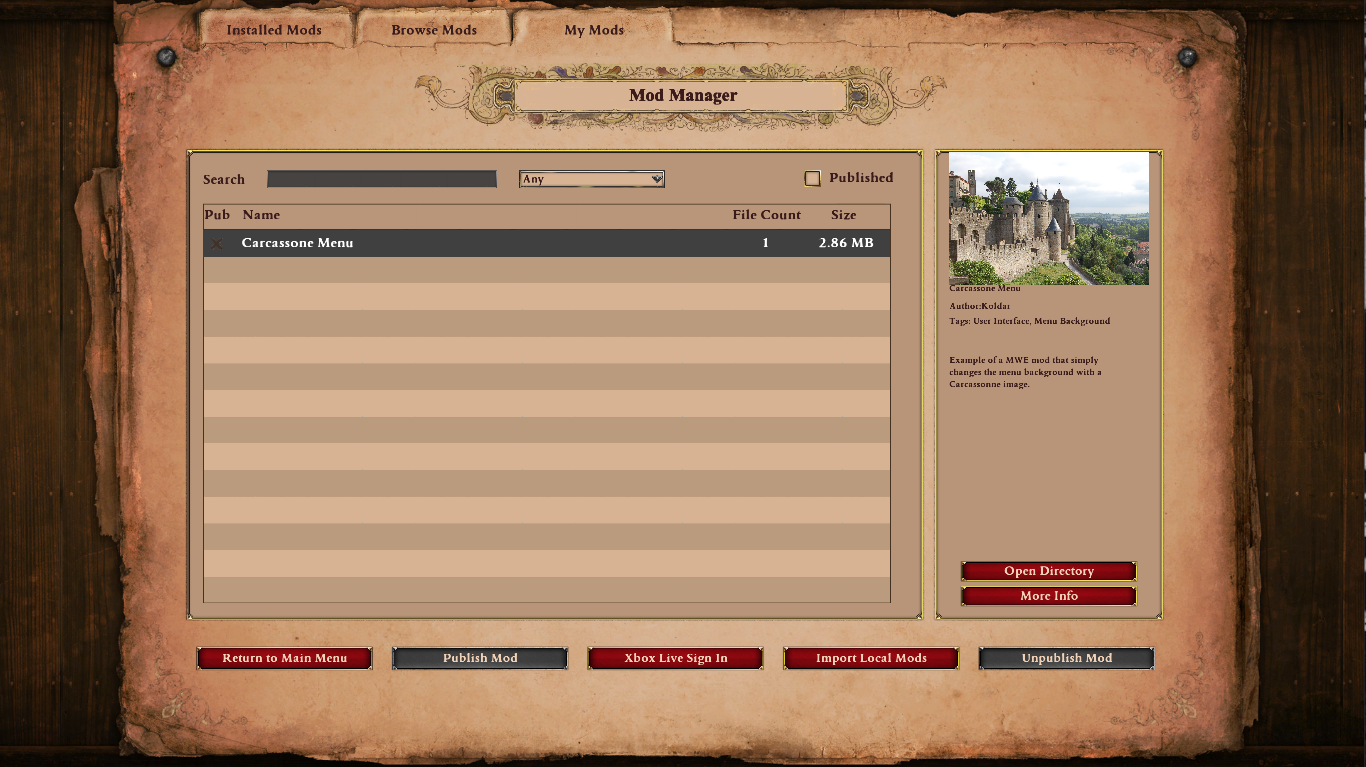
\includegraphics[width=1.0\textwidth]{src/images/mymods}
    \caption{My mods window}
    \label{fig:mymods}
\end{figure}

The image in the background will be clipped. \dquote{mod-status.json} will be automatically updated.

\begin{warning}
    If \code{thumbnail.jpg} is not present, a default image will be put instead. If \code{info.json} is absent, default values will be put: at the moment of writing, the author is set to \dquote{Unpublished}, description to \dquote{No Description} and name as the same folder as the mod root dir. If \dquote{info.json} content is lacking one of those 3 fields, \aoe{} will automatically fill the missing ones.
\end{warning}

In the mod window, if you select the \dquote{carcassonne-menu} you click \dquote{More Info}. If you click this, \aoe{} will automatically open the browser at the \acrref{URL} \url{https://www.ageofempires.com/mods/details/XYZ} where $XYZ$ is the WorkShop Id of the mod. If \aoe{} fails to load the mods, you can \textit{debugging} the mod by make changes the mod in \aoehomelocaldir{} and click \dquote{Import Local Mods} button.

\section{Publish mod}

It is now time to publish the mod. In this way the mod can be automatically downloaded by other client if it is required in a lobby game. In order to publish the mod you need to visit \url{www.ageofempires.com} and sign in with a \textit{XBox Live Account} (Logging with the Steam one is not enough). 

Choose the mod you want to publish and zip the content of the entire mod folder (\ie{} the one containing the file \dquote{info.json} and \dquote{thumbnail.jpg}): this means that if you open the zip file, you will immediately find at the top level the files \dquote{info.json} and \dquote{thumbnail.jpg};\footnote{With \code{7-Zip}, if you right-click the zip and you \dquote{Open} it, you should find such files inside the windows that has just appeared.} then, visit \url{https://www.ageofempires.com/mods/create/} and fill the form with all the required information and finally submit. After some time, you should have published your mode.

Alternatively, you can sign-in inside \aoe{} with you \textit{XBox Live Account}. Then, you can visit te \dquote{My Mods} tab and click on \dquote{Publish Mod} or update when you want to publish a new version of the same mod.

\chapter{Implementing other mods}

In this chapter we describe how to implement some more complex mods.

\section{Altering corpses decaying}

We now try to create a mod that simply changes the time when the corpse decays. Let us call it \textbf{ya-decaying-corpses}.\footnote{\dquote{ya} stands for \dquote{Yet Another} and is a popular way of naming in computer engineering whenever the naming creativity is low.} In this mod, we need to change data files. Data files are located in the \aoeexedir{}\verb|\resources\_common|. As show in Appendix \ref{chp:genieeditor}, you can use \genie{} to do so: Copy the file \aoeexedir{}\verb|\resources\_common\dat\empires2_x2_p1.dat| in the mod dir; then open it via \genie{}. Switch to the \textit{Units} tabs and select all the units of all type (except maybe Gaia's ones). For every one of them, go to the \dquote{Statisitcs} section and change the value \textit{Resource Decay} to \textit{-1}.

\chapter{Creating Random Maps using \acrref{RMS}}

In this chapter we will explain how to use \acrref{RMS} language to generate random maps. For information about \acrref{RMS}, see Appendix \ref{chp:rms} or look at \cite{zetnus:2019}. %We will try to replicate Team Arena by vierklee and the expla.

\subsection{Filling PLAYER\_SETUP}


\clearpage


\backmatter


\begin{appendices}
    \chapter{Semantics of \aoeexedir{}}
    \label{chp:semantics}
    
    \section{BattleServer}

    Folder with \code{BattleServer.exe} file. Usually not useful when modding.

    \section{certificates}

    \code{X509} file format of \aoe{}. Usually not useful when modding.

    \section{Docs}

    Manual of PDF of \aoe{}. Not useful when modding.

    \section{Schema}

    Not useful when modding.

    \section{Support}

    Contains some link to \aoe{} website support. Not useful when modding.

    \section{Tools\_Builds}

    Represents \genie{} directory.

    \section{webclient}

    Not useful when modding.

    \section{wwise}

    Not useful when modding.

    \section{resources}

    Specifies all the data that are not widgets of the \acrref{UI}. The folder contains data like the cursors icons, the \genie{} dat files.

    \subsection{\_common}

    This is the main folder of \textbf{resources} directory.

    \subsubsection{cursors}

    List of all the cursors the cursor directed by the user mouse will display when a given action is performed. For instance, when you need to garrison a villager, a specific cursor image replace the classic arrow icon. All the cursors image have the \code{cur} extension.

    \subsubsection{dat}

    Contains the dat files containing all the information regarding units, civilization, buildings: \code{empires2\_x2\_p1.dat} contains all such information. \footnote{The file can be opened by \genie{}}

    \subsubsection{drs}

    \paragraph{gamedata\_x2}

    This important folder contains \acrref{RMS} files that can be used in your \acrref{RMS} programming (\eg{} \code{F\_Season.inc}). See Appendix \ref{chp:rms}.

    \section{widgetui}

    Specifies which set of textures \aoe{} needs to display alongside their configuration. If you need to alter a picture, it will probably be here.
    Contains a set of json.
    Furthermore, it contains a folder named \dquote{textures}, representing all the textures and images in the game. There are versions, \textit{textures} and \textit{textures-sd}: the former contains the texture to use and the latter contains the low resolution version of the same textures. The first texture are mandatory while the second are optional (modwise). All textures are saved via \acrref{DDS} extensions.\footnote{You can use \code{Irfan View} 32-bit version to view \acrref{DDS} images.}

    \code{Textures} folder contains other folders:

    \subsection{atlas} 

    Contains textures that are present in the Campaigns menu (\eg{} the scenes where you can choose which campaign to play), Sun Tzu icons in the \dquote{Art of War}, images representing the \acrref{UI} you see while playing (\figref{fig:CivAsia}), the window chat, buildings icons (\figref{fig:ingamebuildings}).

    \begin{figure}
        \centering
        \begin{subfigure}{0.48\textwidth}
            \centering
            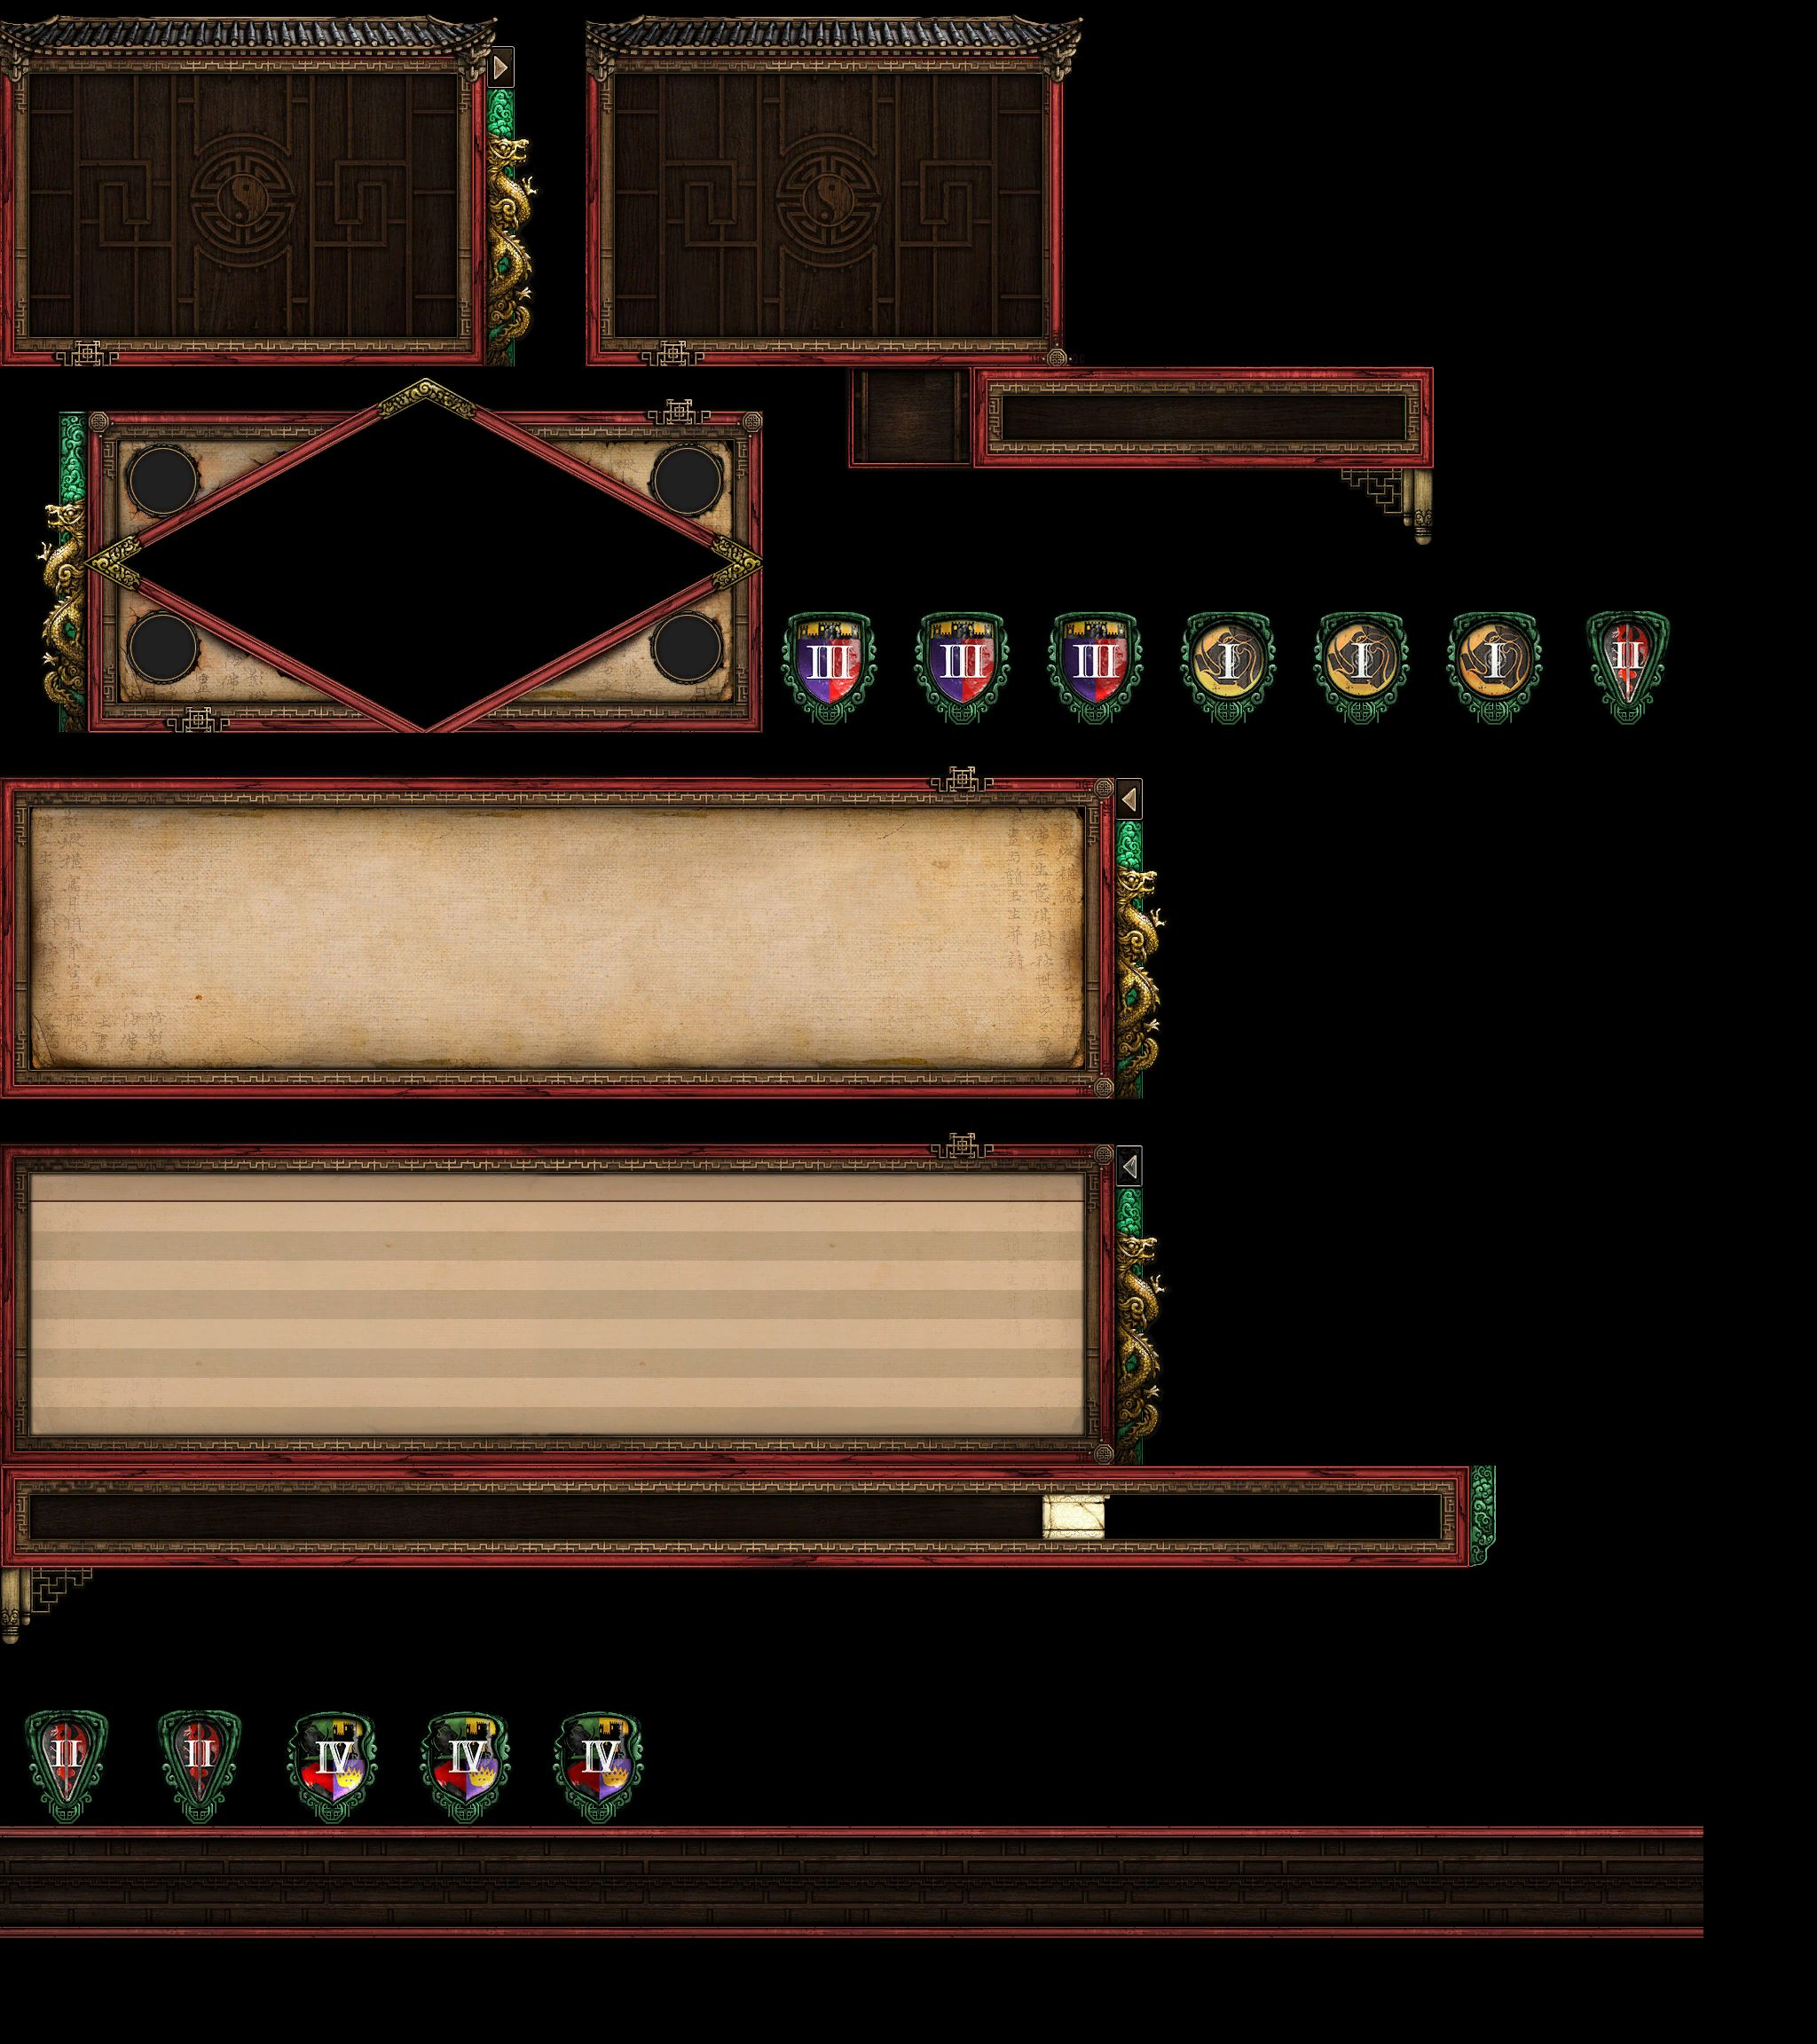
\includegraphics[width=1.0\textwidth]{src/images/CivAsia}
            \caption{CivAsia file, containing the \acrref{UI}}
            \label{fig:CivAsia}
        \end{subfigure}\quad%
        \begin{subfigure}{0.48\textwidth}
            \centering
            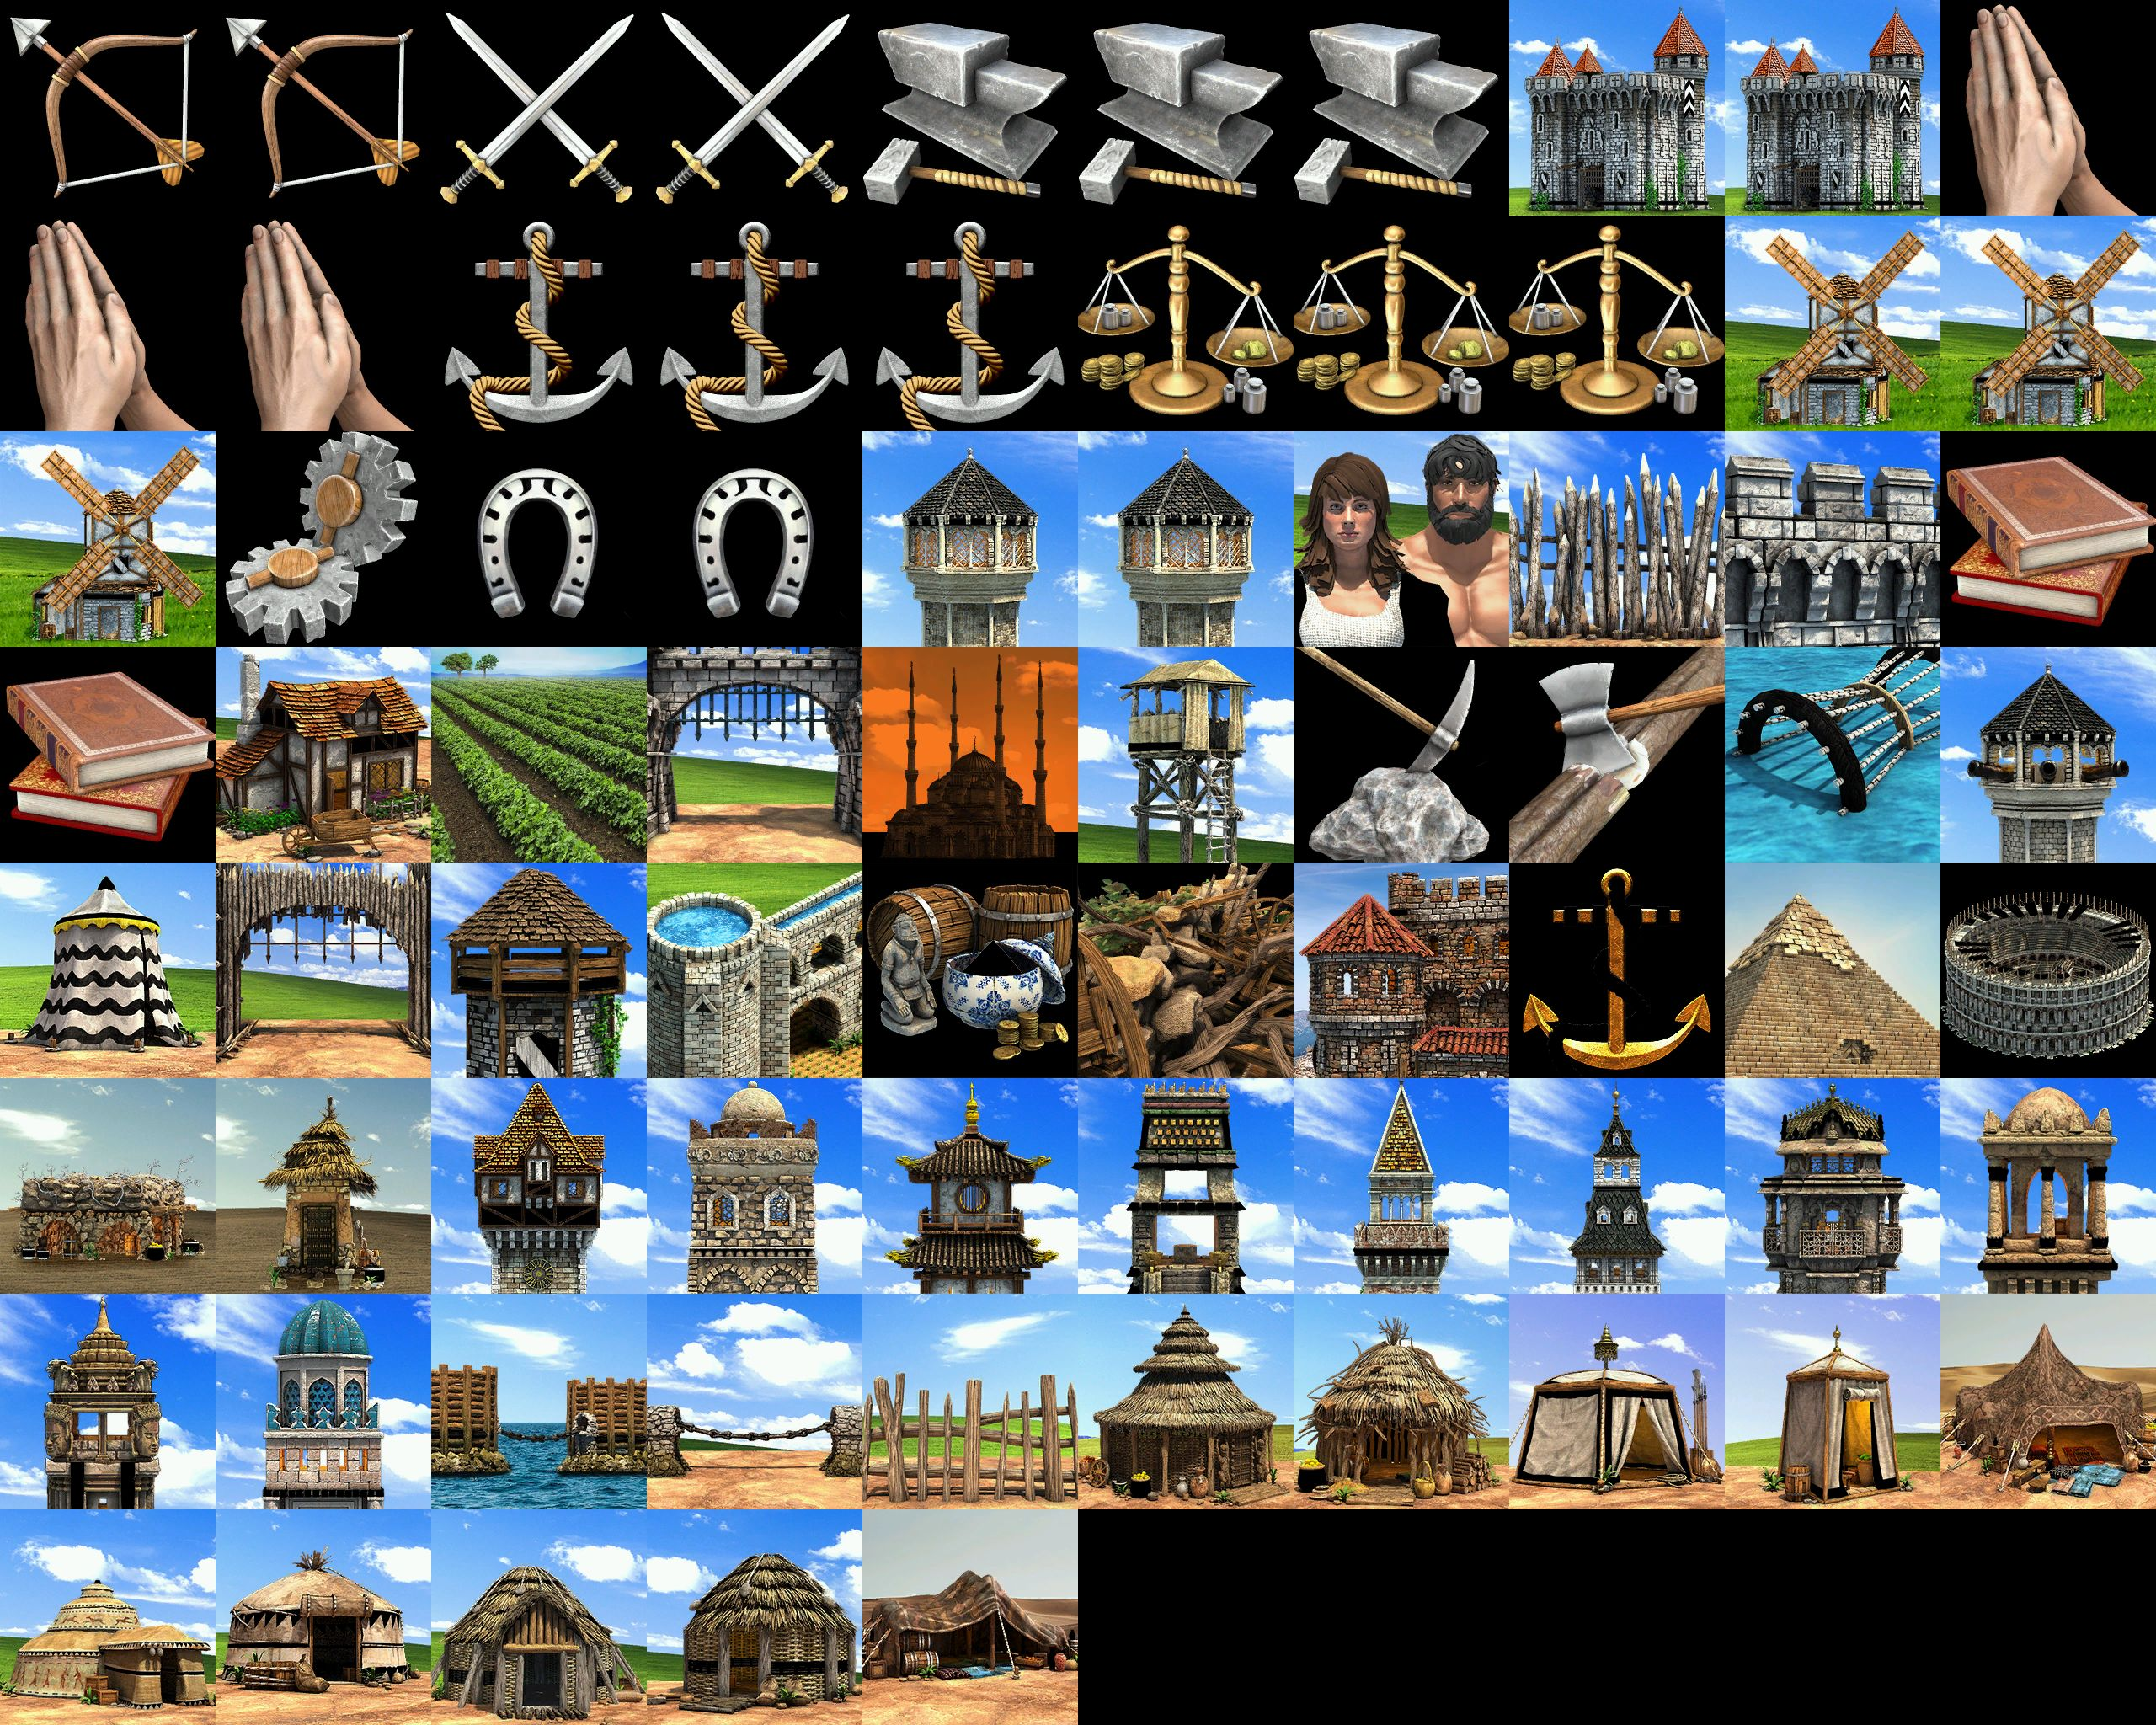
\includegraphics[width=1.0\textwidth]{src/images/ingamebuildings}
            \caption{ingamebuildings file, containing the icons of the buildings in \acrref{UI}}
            \label{fig:ingamebuildings}
        \end{subfigure}\\%
    \end{figure}

    \subsection{backgrounds}

    Contains the menu background (\dquote{mainmenu\_bg} and \dquote{mainmenu\_bg\_1}) images as well the windows in the \aoe{} menus (\eg{} lobby creation, history). Examples of these figures are shown in \figref{fig::backgrounds}. Note that some of images here are represented via \acrref{PNG} rather than \acrref{DDS}.

    \begin{figure}
        \centering
        \begin{subfigure}{0.48\textwidth}
            \centering
            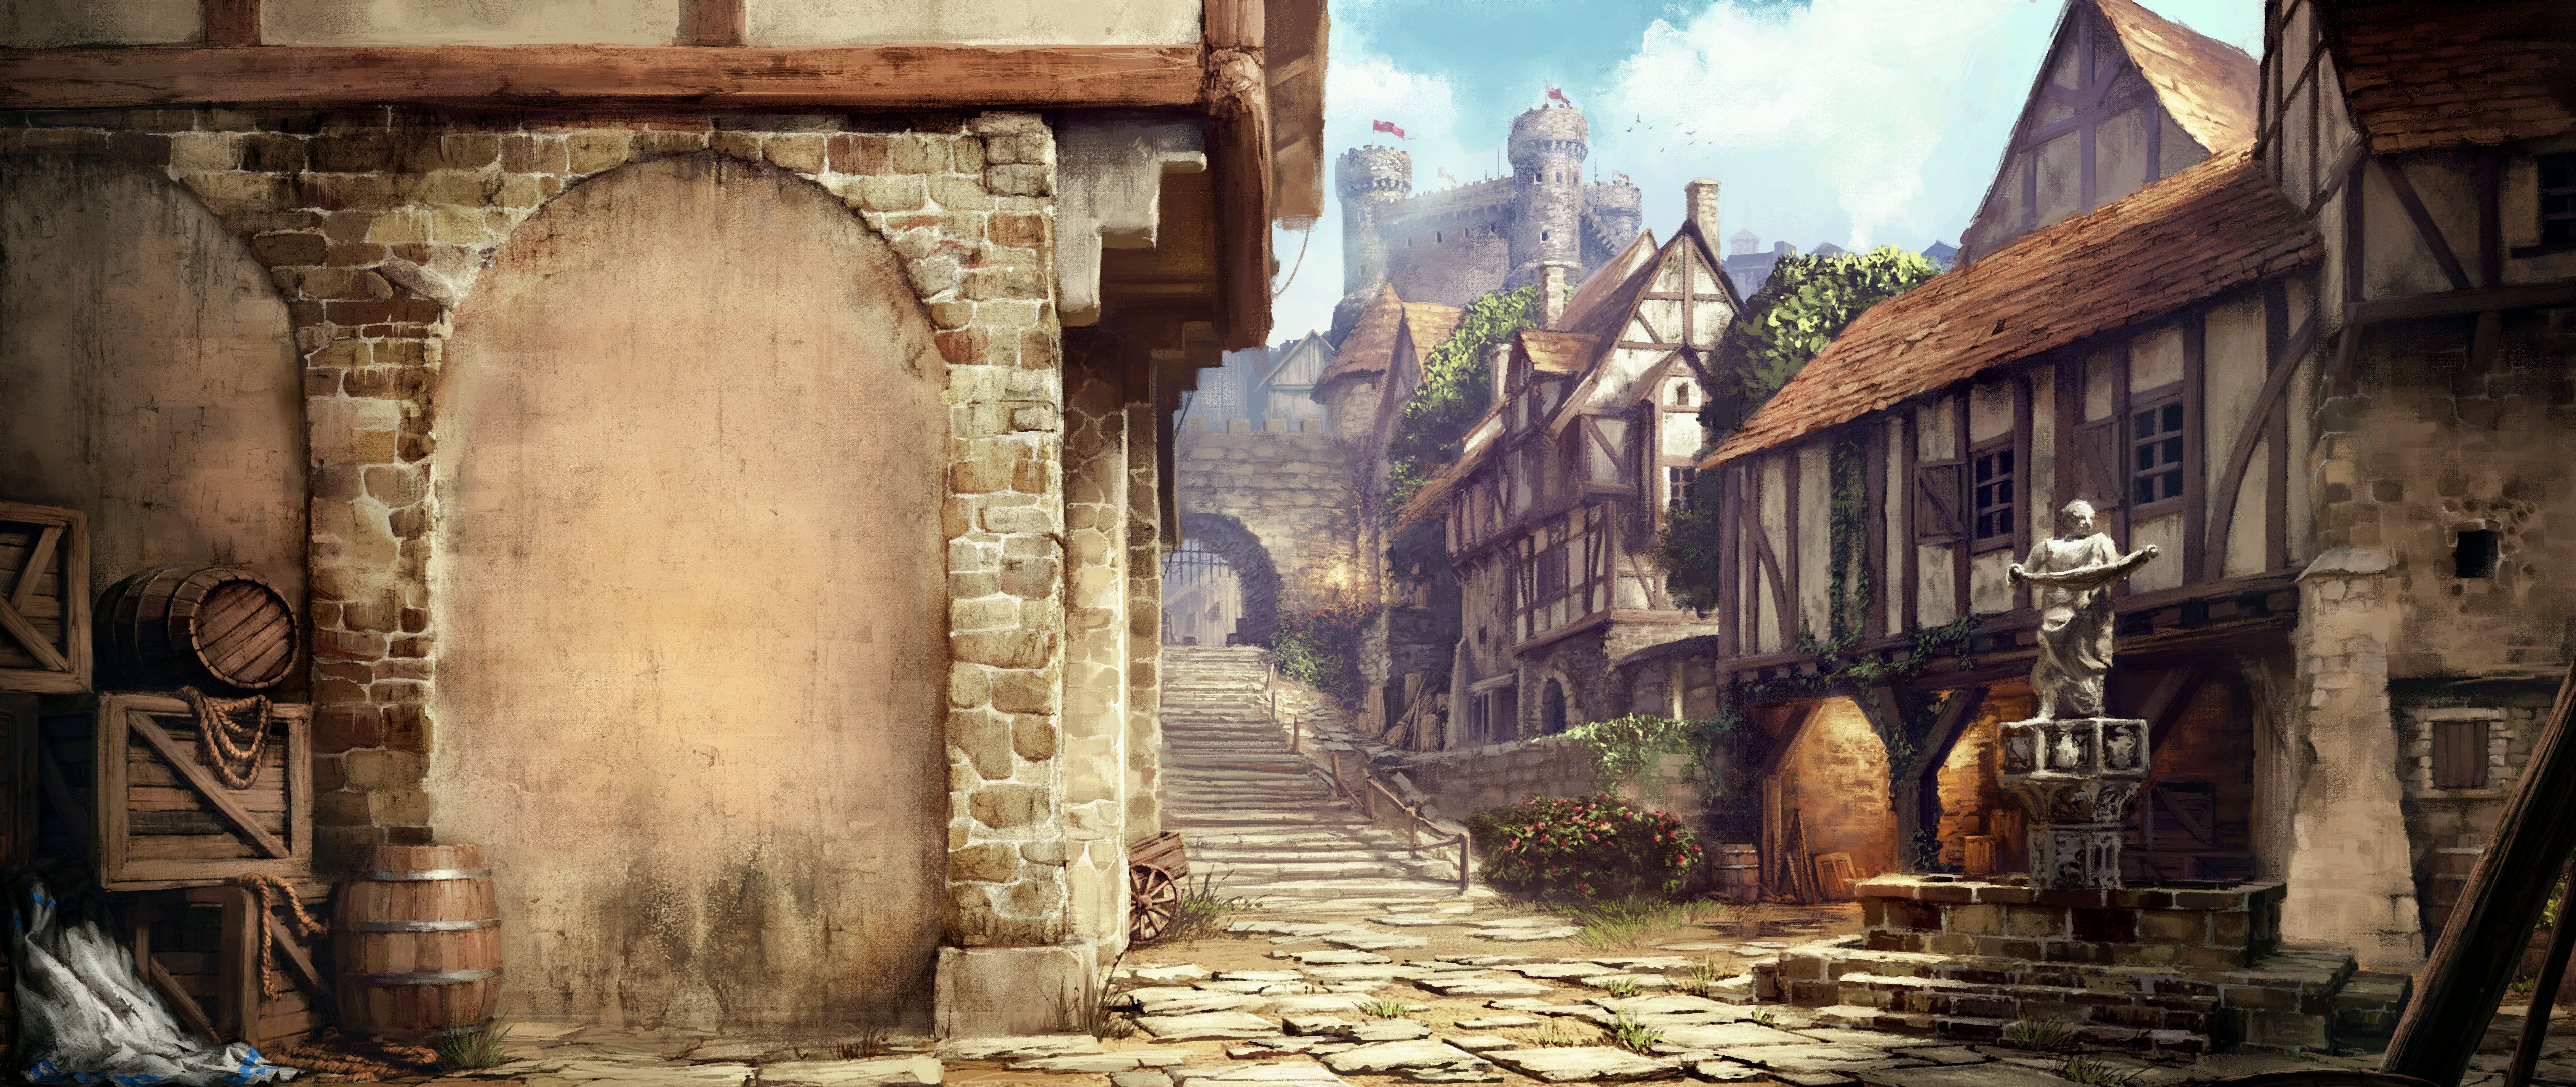
\includegraphics[width=1.0\textwidth]{src/images/mainmenu-bg}
        \end{subfigure}\quad%
        \begin{subfigure}{0.48\textwidth}
            \centering
            
\includegraphics[width=1.0\textwidth]{src/images/popup-menu-bg}
        \end{subfigure}\\%
        \caption{Background menu examples}
        \label{fig:backgrounds}
    \end{figure}

    \subsection{campaign}

    Texture regarding the campaigns, one sub directory per campaign. For instance, \dquote{cam3} is the \textit{Saladin Campaign}. Within it:
    \begin{itemize}
        \item $X.dss$ file, where $X$ is the campaign name, is the campaign image menu file (\ie{} the image where you can choose the specific mission);
        \item $X$\_$background$ is the image where the mission intro and outro are presented;
        \item a subfolder, one per mission in the given campaign. Each sub folder name has a number (starting from 1) as name and contains the drawings in the intro and outros of the associated mission.
    \end{itemize}

    \subsection{ingame}

    TODO

    \subsection{menu}

    TODO
    \chapter{Advance Genie Editor}
    \label{chp:genieeditor}

    This is a small guide to \genie{} software. The guide is based on version 2020.3.30. You should not consider this guide as something as official. \genie{} is a program for editing data of genie (\acrref{DAT} and \acrref{DLL}) files. It can edit properties of units, civilizations, technologies, graphics, terrains, sounds, player colors and some other things\cite{TurnupHyperion4:2019}.
    \genie{} program can be found in \aoeexedir{}, under \dquote{Tools\_Build} directory.

    When you execute it three windows automatically open. The \textit{Open files...} allows you to open a \genie{} file. To manage \aoe{} files, click on the button \textit{Age of Empires II: Definitive Edition} on the right of \textit{Defaults:} label. Set the \textit{Genie version:} to \textit{Age of Empires II: Definitive Edition}.
    The file that you need to open is the one specified by \textit{Compressed data set (*.dat)}: such a file should be called \code{empires2\_x2\_p1.dat}. When you open such a file you can view all the unit, buildings, civilizations parameters and properties. The vanilla file is \code{C:\textbackslash{}Program Files (x86)\textbackslash{}Steam\textbackslash{}steamapps\textbackslash{}common\textbackslash{}AoE2DE\textbackslash{}resources\_common\textbackslash{}dat\textbackslash{}empires2\_x2\_p1.dat}.

    After opening the file, you can now make changes on the file. \figref{fig:genie01} shows the state fo the program when it opens the file. 

    \begin{figure}[ht]
        \centering
        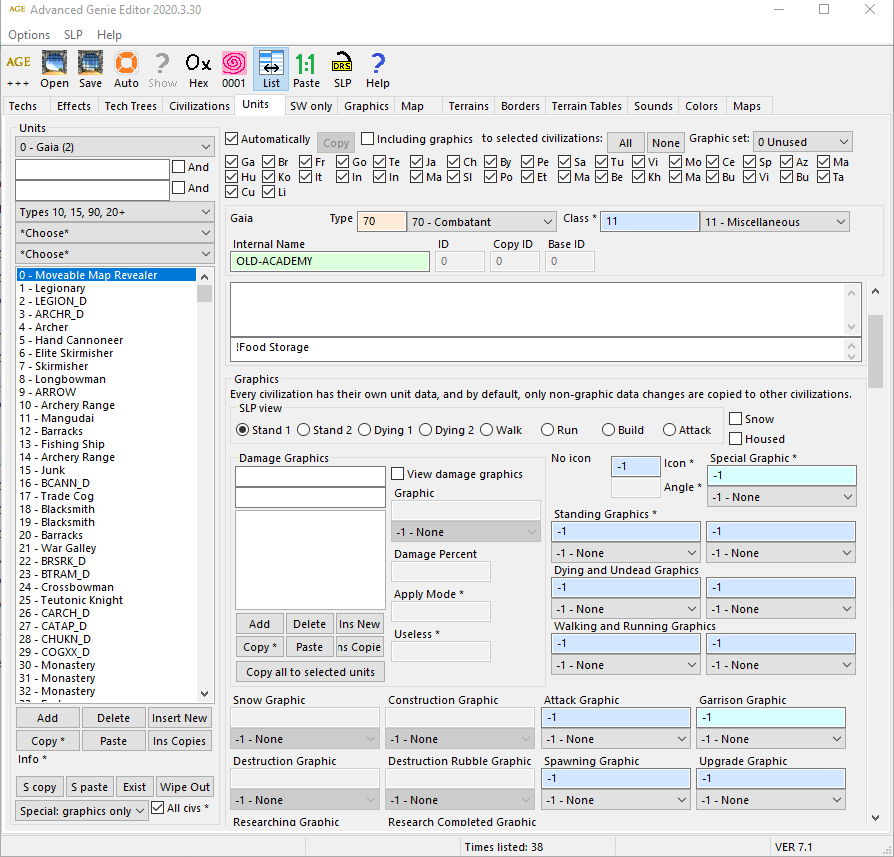
\includegraphics[width=0.7\textwidth]{src/images/genie01}
        \caption{Standard \genie{} window}
        \label{fig:genie01}
    \end{figure}

    As shown in \figref{fig:genie03}, \genie{} splits its parameters regarding the \aoe{} field.

    \begin{info}
        You can switch between tabs by the performing hotkeys \code{Ctrl + Pag. Up} and \code{Ctrl + Pag. Down}.
    \end{info}

    \begin{figure}[ht]
        \centering
        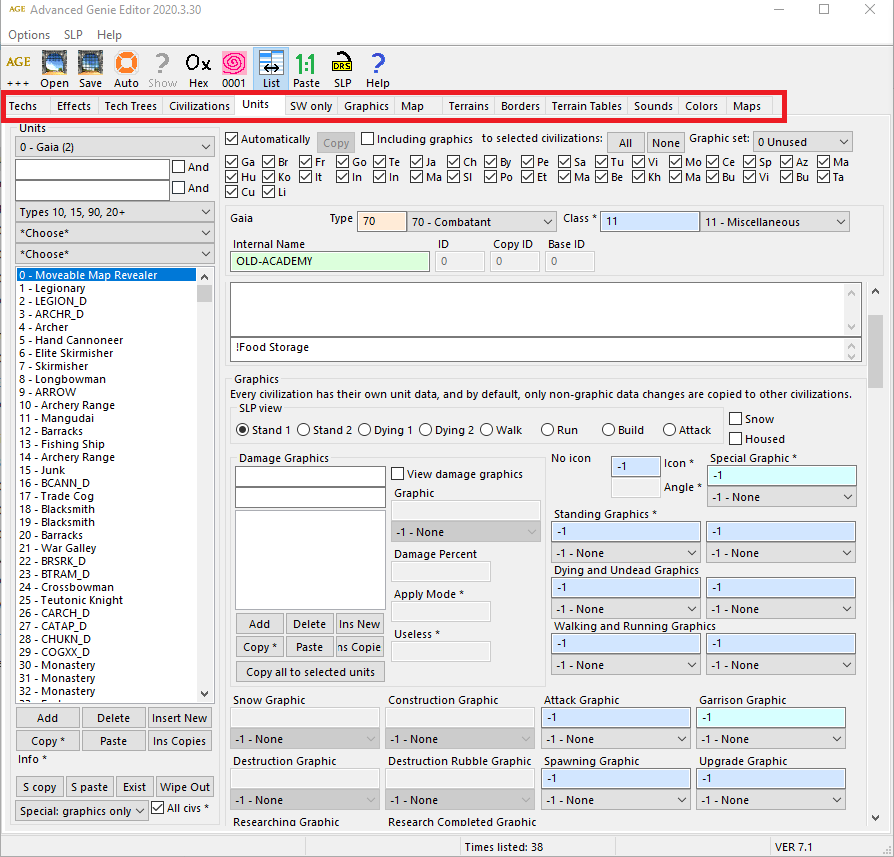
\includegraphics[width=0.7\textwidth]{src/images/genie03}
        \caption{Standard \genie{} window. The red box highlights the category tabs grouping the parameters you can tweak according to the \aoe{} field.}
        \label{fig:genie03}
    \end{figure}

    In the units left pane (called \dquote{Units}) there is displayed the list of all the units a particular civilization can manage (\eg{} in \figref{fig:genie02} the civ is \dquote{Gaia}). Since the unit tabs show several parameters and unit, you can filter the units using the search box in the units pane (\eg{} \figref{fig:genie02} highlighted in the red box).

    \begin{figure}[ht]
        \centering
        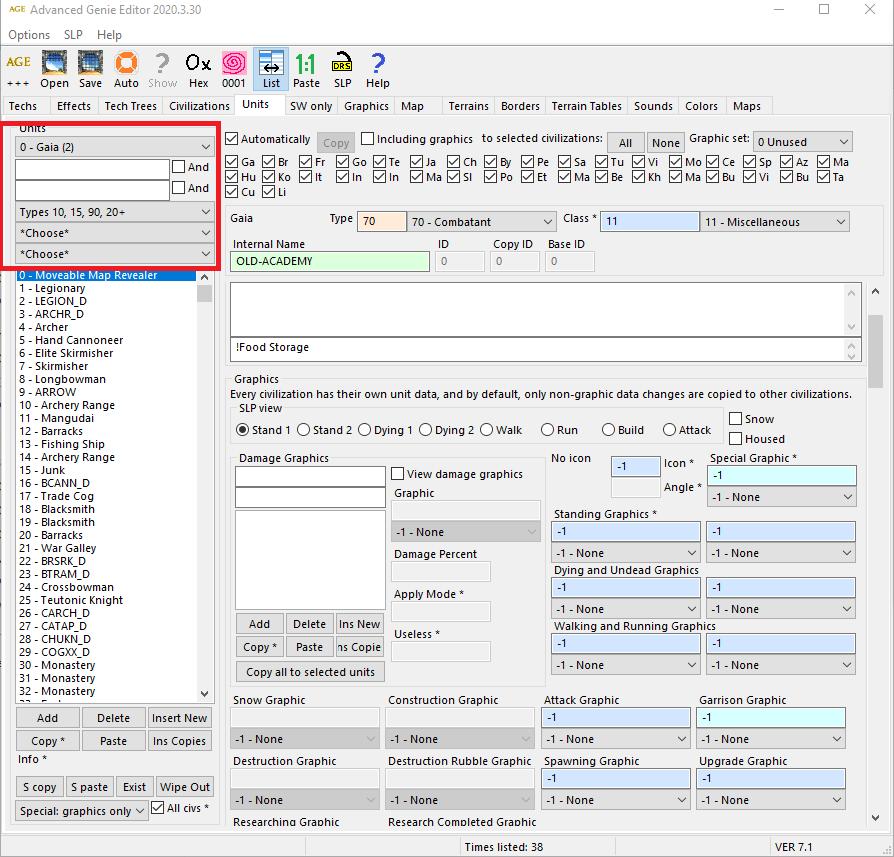
\includegraphics[width=0.7\textwidth]{src/images/genie02}
        \caption{Standard \genie{} window. The red box highlights the search boxes you can use to filter }
        \label{fig:genie02}
    \end{figure}

    The search box works as follows: first you select the civilization, then you can add at most 2 criteria involving the unit name (in and with the civilization): namely, if the 2 criteria are $\gamma_1$ and $\gamma_2$ and the civilization involved is $c$, the whole search criterion is $civ = c \land (\gamma_1 \in unit.name) \land (\gamma_2 \in unit.name)$, where $unit.name$ is the string representing a generic unit name. For instance, if $\gamma_{1} = dead$ then we select all the units whose name contains the substring \dquote{dead}. You can add \dquote{|} to perform a logical or ($\squote{\lor}$) inside $\gamma_{i}$ ($i \in \{1,2\}$). For instance if $\gamma_{1} = \_D|dead$, the global search criterion is $civ = c \land ((\_D \in unit.name) \lor (dead \in unit.name))$: such a search query will generate all the units whose name contains either \dquote{\_D} or \dquote{dead}.

    You can select multiple units: when you alter a value from the unit pane, the same parameter will be updated also in every other civilization checked in the top checkboxes (\eg{}, \dquote{Ga}, \dquote{Br}, \dquote{Fr}, \dquote{Go}). At the bottom you can see how many changes performed in this session (as shown in \figref{fig:bottombar}).

    \begin{figure}[ht]
        \centering
        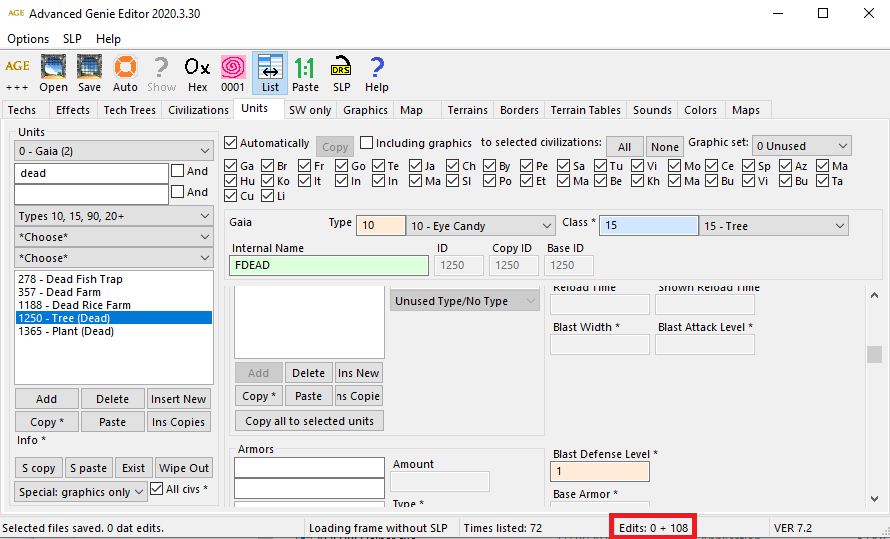
\includegraphics[width=0.8\textwidth]{src/images/bottom-bar}
        \caption{Example of how the bottom bar can be used to check how many changes we have made so far.}
        \label{fig:bottombar}
    \end{figure}

    \section{Required Knowledge}

    \paragraph{Unit names.}
    The units ending with \dquote{\_D} represent the corpses of the associated unit: for instance \dquote{Archer} unit is the actual unit with all its properties while \dquote{ARCHR\_D} represents the archer corpse.

    \paragraph{Buildings.} Every time the user access to a new era, each building changes. For instance, in \textit{graphics} you can see that there are, for each stable building civ, a stable for feudal, one for the castle age and another one for the imperial age.

    \section{Units parameters}

    Manage a single unit parameters. This section is divided in multiple sub areas:

    \begin{itemize}
        \item Language Files;
        \item Graphics;
        \item Statistics;
        \item Projectiles;
        \item Attributes;
        \item Sounds;
        \item Tasks;
    \end{itemize}

    The documentation in this area has been copied from \cite{agewiki:2014}.

    \subsection{Language Files}

    \subsection{Graphics}

    \subsection{Statistics}

    \textbf{Hit Points}: hit points of the unit. If -1, the unit will immediately die\cite{genie:hitpoints}. \textbf{Speed}: the speed of the unit. \textbf{Rotation Speed} makes the unit slower. \textbf{Line of Sight} represents the number of cells the unit can see. Generates a circle centered in the unit. \textbf{Search Radius} is determines the area within which the unit will recognizes and react to other units.  If anything enters this area, the unit will notice it; If you enter a value higher than LOS, a unit will chase enemy units outside of its sight range. \textbf{Min Range} (\textbf{max Range}) represents the minimum (maximum) range the ranged unit can shoot its projectile: for example an archer can shoot any target between 0 and 4 cells\cite{agewiki:2014}.

    \textbf{Resource capacity} determines the quantity of resources a unit can hold (in range $[0, 3392]$): for villagers, this is the max amount of resources they can carry. For other units, it can be other resources, like the time it takes for a dead unit to decompose\cite{agewiki:2014}.

    \textbf{Resource Decay} determines how fast objects (like corpses) decay. Set -1 for never decaying. A negative value will prevent the corpse from decaying permanently. The larger a positive value is, the longer the corpse will last. (The value is approximately the equivalent number of game seconds). Many non-corpse units have resource decay value, but the purpose of it in other units is unknown\cite{agewiki:2014}. 

    \textbf{Work Rate} determines the base work speed of units. This affects rates like villager work rates (building, gathering, etc.), conversion speed, and trebuchet pack (unpack) speed. the value needs to satisfy the constraint $x \geq 0$\cite{agewiki:2014}.

    \textbf{Garrison Capacity} is the number of units a transport or building can hold. allowed value $x$ must satisfy the constraint $x \in [-1, 127]$. Only rams, buildings, and transport ships can normally hold units. \footnote{Garrisoning infantry into rams will increase both the ram's speed and attack.} If you give a rams an original speed of 0, garrisoning units will allow it to move. 

    \textbf{Garrison type} determines what units can garrison into the building ($x \in [0, 15]$). Such a integer value should be interpreted as an enumeration, which semantic is shown in \tblref{tbl:garrisontype}. The number are encoded in \genie{} as a 8-bit value\cite{agewiki:2014}.

    \begin{table}[ht]
        \centering
        \begin{tabular}{ll}
            \toprule
            Value & Semantic \\
            \midrule
            0   &   None \\
            1  &  Villagers only \\
            2  &  Infantry only \\
            3  &  Villagers and infantry \\
            4  &  Cavalry \\
            5  &  Cavalry and villagers \\
            6  &  Cavalry and infantry \\
            7  &  Cavalry, infantry and villagers \\
            8  &  Monks only \\
            9  &  Monks and villagers \\
            10  &  Monks and infantry \\
            11  &  Monks, infantry and villagers \\
            12  &  Monks and cavalry \\
            13  &  Monks, villagers and cavalry \\
            14  &  Monks, cavalry and infantry \\
            15  &  Monks, villagers, infantry and cavalry \\
            \bottomrule
        \end{tabular}
        \caption{Semantic of each Garrison Type value.}
        \label{tbl:garrisontype}
    \end{table}

    \textbf{Garrison Heal Rate} determines how fast a building heals units garrisoned within it ($x \geq 0$). This is different from the Garrison Recovery, which determines how fast the unit heals when garrisoned in any building\cite{agewiki:2014}.

    \subsection{Projectiles}

    \subsection{Attributes}

    \textbf{Dead Unit} Represents the unit representing the corpse of the unit currently under analysis. By convention, all \dquote{dead units} ends with \code{\_D}. If a unit does not have any dead unit, this field is set to $-1$. For example, the dead unit of the unit \dquote{Archer} is set to be \code{ARCHR\_D} unit.

    \subsection{Sounds}

    \subsection{Tasks}

    \section{Graphics}

    Represents the graphics and the animations involved in every units and buildings. This section has been copied from \cite{agewiki:grpahics:2014}. The left pane represents the sprites of each unit, building and so on. There is a search box that is similar to the one in \dquote{Units}.

    \textbf{Internal Name} is the name used to identify the sprites in the \genie{} in the left pane of \dquote{Graphics} panel.

    \textbf{Frames per Angle} represents the framerate of the sprite.

    \textbf{Animation Duration} represents how long the animation is displayed in seconds. After that time the animation stops and the sprite is removed. It is required that $x > 0$. Exponential notation can be used (\eg{} $e3+35$). Use this field if you want to avoid the sinking of dead units for every sprite whose name contains \dquote{(Decay)} substring. If the duration input is larger than the actual animation length, 

    \subsection{Deltas}

    The deltas section allows to combine multiple sprites togther ina single animation. The sprites and animation that are combined are the one shown in the left pane (see \figref{fig:deltas}).

    \begin{figure}[ht]
        \centering
        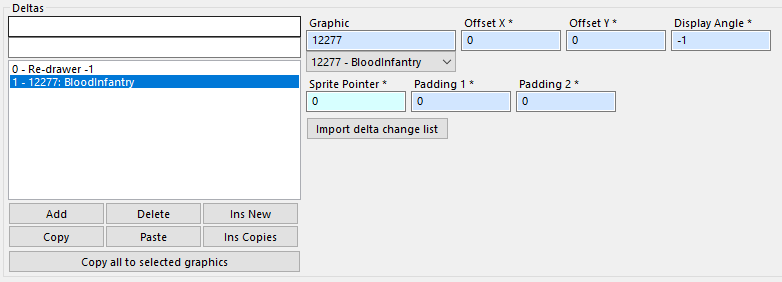
\includegraphics[width=1.0\textwidth]{src/images/deltas}
        \caption{Section of Graphics allowing you to combine different textures together.}
        \label{fig:deltas}
    \end{figure}

    \textbf{Graphic} represents the id of the sprite to show. The name of the file refers to the json file present in \code{resources/\_common/particles}.

    \textbf{Padding 1} and \textbf{Padding 2} are not useful.

    \subsection{Angle Sounds}

    
    %On the top _D|dead \cite{gagmanAoC:2017}
    \input{src/texs/83-appendix-rms-file-format.tex}
\end{appendices}


\printglossary[type={terms}]
\clearpage
\backmatter

\bibliographystyle{unsrt}
\bibliography{src/bibs/biblio}
%to use multiple biblios
%\bibliography{src/bibs/csp, src/bibs/pathfinding}


\end{document}
